\documentclass[12pt,a4paper]{book}

%load some useful latex packages
\usepackage{alltt}    %tt mode for sequences etc
\usepackage{lscape}   %landscape mode
\usepackage[ngerman,english,french]{babel} % set the amazing french language
\usepackage{fontspec} %use all fonts
\usepackage{titlesec} %redefine titles
\usepackage{fancyhdr} %fancy headers 
\usepackage{xcolor}   %colors
\usepackage{graphicx} %graphics
\usepackage{amsfonts} %more sophisiticated math symbols
\usepackage{siunitx}  %alignement in tables
\usepackage{listings} %use code listings
\usepackage{url}
\usepackage[nottoc,numbib]{tocbibind} %add bibliography to TOC

%load some useful colors
%able to read on white
%blue
\definecolor{a-aqua}    {rgb}{0,0.5,1}      
%red
\definecolor{a-salmon}  {rgb}{1,0.4,0.4}
%green
\definecolor{a-flora}   {rgb}{0.4,1,0.4}
%purple
\definecolor{a-lavender}{rgb}{0.8,0.4,1}
%orange
\definecolor{a-tangerine}{rgb}{1,0.5,0}
%gray
\definecolor{a-aluminium}{rgb}{0.6,0.6,0.6}
%brown
\definecolor{a-mocha}    {rgb}{0.5,0.25,0}
%unable to be clearly read on white
\definecolor{a-sky}     {rgb}{0.4,0.8,1}
\definecolor{a-banana}  {rgb}{1,1,0.4}

\lstset{
  basicstyle =\scriptsize\ttfamily,
  showspaces = false,
  showstringspaces = false, 
  showtabs = false, 
  captionpos =b, 
  keywordstyle = \color{a-aqua},
  commentstyle = \color{a-flora},
  stringstyle = \color{a-salmon}
}


%Basic font layout
\setsansfont{DejaVu Sans}
\setmainfont{DejaVu Serif}
\setmonofont{DejaVu Sans Mono}

\newfontfamily\chapterfont{DejaVu Sans ExtraLight}

%titles
\titleformat{\chapter}[hang]{\Huge\chapterfont\color{a-aqua}}{\thechapter\hspace{5mm}{|}\hspace{5mm}}{0pt}{\Huge\chapterfont\color{a-aqua}}
\titleformat*{\section}{\Large\sffamily\color{a-aqua}}
\titleformat*{\subsection}{\large\sffamily\color{a-aqua}}
\titleformat*{\subsubsection}{\sffamily\color{a-aqua}}

%Headers and footers
\pagestyle{fancy}
\renewcommand{\headrulewidth}{0pt}
\renewcommand{\footrulewidth}{0pt}
\lhead[]{\scriptsize\leftmark}
\rhead[\scriptsize\rightmark]{}
\lfoot[]{\scriptsize\thepage}
\rfoot[\scriptsize\thepage]{}
\cfoot[]{}

\fancypagestyle{plain}{
\fancyhf{}
\renewcommand{\headrulewidth}{0pt}
\renewcommand{\footrulewidth}{0pt}
\lfoot[]{\scriptsize\thepage}
\rfoot[\scriptsize\thepage]{}
}

%hyphenation
\hyphenation{
meth-yl-a-cet-a-mide
mol-e-cule
mol-e-cules
}

\begin{document}

\selectlanguage{english}
%table of contents
\tableofcontents

%redefine openleft
\makeatletter
\renewcommand*\cleardoublepage{\clearpage\if@twoside
  \ifodd\c@page \hbox{}\newpage\if@twocolumn\hbox{}%
  \newpage\fi\fi\fi}
\makeatother

%inputs of the actual chapters
\chapter{Introduction}

This manual is written as a guide for scientists using and continuing to
develop \emph{MNHN-Tools}. As such this guide provides you with a
installation procedure, detailed usage instructions and technical
details for every tool contained within this suite and a tutorial to get
the reader started with a typical clustering and density distance
based phylogenetics as well as tree building.

\section{License}
Copyright (C) 2019-2020 Thomas Haschka \newline
This software is provided 'as-is', without any express or implied
warranty.  In no event will the authors be held liable for any damages
arising from the use of this software.

Permission is granted to anyone to use this software for any purpose,
including commercial applications, and to alter it and redistribute it
freely, subject to the following restrictions:

\begin{enumerate}
  \item The origin of this software must not be misrepresented; you must not
    claim that you wrote the original software. If you use this software
   in a product, an acknowledgment in the product documentation would be
   appreciated but is not required.
  \item Altered source versions must be plainly marked as such, and must not be
    misrepresented as being the original software.
  \item This notice may not be removed or altered from any source,
    binary distribution and this manual.
\end{enumerate}

\section{General Overview}

\emph{MNHN-Tools} was developed in order to cluster and infer
phylogenetic evolution into repeated sequences in a single genome,
namely: α-satellites in primate genomes. During the development
the versatility of the tools presented herein was both discovered and
enforced. As such this tool is applicable to all kinds of data
discovery tasks on datasets of sequences. Notebly this tool has been
used for experiances around Deoxyribonucleic Acid (DNA) barcoding tasks
Operational Taxonomic Unit (OTU) detection.

\emph{MNHN-Tools} is a suite that allows you to gain insights
into a dataset composed of nucleic or protein sequences provided as
FASTA \cite{fasta} files. The tool has the ability to cluster such a
dataset and to built phylogenetic trees based on a density- distance
based criteria. This is achieved by a repeated application of the
Density-Based Spatial Clustering of Applications with Noise (DBSCAN)
\cite{dbscan} algorithm. Clustering and gaining such sequence-sequence
dependency or phylogentic insights are at the heart of this
software. Nevertheless this software provides you with all kinds of
tools that might be of use, such as, but not limited to: The
generation of fasta datasets using simulated evolution, the projection
of FASTA files into a Principal Component Analyses (PCA) based subspace, the
evaluation of k-mer vectors from fasta datasets or the calulation of
clustering parameters such as the Silhouette \cite{silhouette}
index on a dataset.

\chapter{Installation}

In this chapter we will provide you with the details that allow you to
install \emph{MNHN-Tools}. The primary distribution method is in the
form of source code on github: \newline
\url{https://github.com/haschka/mnhn} \newline

For a full installation a machine with a UNIX or UNIX-like system
is required. The machine currently has to be of \emph{x86\_64}
architecture and support the \emph{AVX} instruction set. In order to
compile the full suite of tools you need a toolchain, consisting of:
\begin{itemize}
\item \emph{make:} Which is required to build the suite and various subsets
\item \emph{compiler/linker:} A working C compilier, the suite was found to
  compile with \emph{gcc} and \emph{clang}.
\item \emph{BLAS/LAPACK} An implementation of the BLAS/LAPACK
  libraries.
\item \emph{OpenCL:} A working implementation of the OpenCL
  language. The suite was tested to compile with the
  \emph{nvidia-opencl-toolkit} or the \emph{intel-opencl-sdk}.
\item \emph{SDL2:} An implementation of the SDL2 library.
\item \emph{MPI:} An implementation of the Message Passing Interface
  (MPI). The suite was tested with \emph{OpenMPI}.
\item \emph{PNG:} An implementation of the PNG graphics library.
\end{itemize}
You may make sure that you not only have the binary versions of the
supporting libraries installed but also the header files, otherwise
the software will not be able to compile. As such you may need to
install the developer \emph{-dev} versions of the libraries. In the
next step you may clone the \emph{MNHN-Tools} source code from github.
You can do this by issuing the following command in your UNIX
terminal:
\lstset{language=bash,
  caption={Cloning the source from github.},
  label=lst-git-clone}
\begin{lstlisting}                                                              
git clone https://github.com/haschka/mnhn.git
cd mnhn
\end{lstlisting}
Cloned and enterd the mnhn directory you need to edit the head of the
make file suite your UNIX systems needs, select the correct compiler
flags and linking commands to the libraries. You may consult the
forums and documentation of your System/Distribution to find the
correct values. In general \emph{CC} is the command of your compiler,
\emph{MPICC} the MPI wrapper of your compilier. \emph{CFLAGS} the
options that you want to pass to your compilier. The other options are
the linker flags to the corresponding libraries.
\lstset{language=make,
  caption={Heat of the Makefile},
  label=lst-make-head}
\begin{lstlisting}                                                           
CC=gcc
MPICC=mpicc
CFLAGS= -O2 -march=native -ftree-vectorize -fomit-frame-pointer 
LAPACK=-llapack
MATH=-lm
PTHREAD=-pthread
OPENCL=-lOpenCL
PNG=-lpng
MPI=-lmpi
SDL=$(shell sdl2-config --cflags) $(shell sdl2-config --libs)
\end{lstlisting}
With your flags adjusted you may compile the code issuing
\lstset{language=bash,
  caption={Building all tools},
  label=lst-build}
\begin{lstlisting}
mkdir bin
make all
\end{lstlisting}
If you do not need the full functionality of \emph{MNHN-Tools} you can
install each tool individually by calling:
\lstset{language=bash,
  caption={Building individual tools},
  label=lst-make-head-individual}
\begin{lstlisting}
mkdir bin
make name-of-the-tool
\end{lstlisting}
This might especially be convenient if you are not able to install all
the libraries in question on your system as the tool that you might
really need might not depend on the library that you might not be able
to install.

\chapter{Tools}

In this chapter we describe each tool in detail, how to use it, the
algorithm used to implement it, and algorithmic specifities.

\section{fasta2kmer} \label{sec-fasta2kmer}

\subsection{General}

The \emph{fasta2kmer} tool implements the calculation of k-mer
frequencies for each sequence to be found in a FASTA \cite{fasta}
file. The tool can calculate both k-mer frequencies for nucleic and
protein sequences. k-mers are all possible sequences for k
letters. The frequencies tell how often each of these k-mers is found
in the entire sequence.

\subsection{Usage}

\lstset{language=bash,
  caption={Calling the \emph{fasta2kmer} tool},
  label=lst-fasta2kmer-call}
\begin{lstlisting}
fasta2kmer [fasta-file] [kmer-length] [number-of-threads] [protein?] > kmerbase
\end{lstlisting}
The \emph{fasta2kmer} tool has the following arguments:
\begin{enumerate}
  \item \emph{fasta-file} The FASTA file containing the sequences to
    calculate k-mer frequencies of.
  \item \emph{kmer-length} The length of the k-mers to calculate
    frequencies from.
  \item \emph{number-of-threads} The number of individual threads to
    be available for this computation. A good choice is the number of
    logical cores available on the machine in question.
  \item \emph{protein?} Set 0 for nucleic sequences, 1 for protein
    sequences.
  \item \emph{kmerbase} The output file to write kmer frequencies
    for each sequence to. The format of this file is tabulator
    separated. The first entry in each line is 
    \emph{sequence\_N} where N is the sequence number attributed
    counting from 0 to N by occurrence of sequences in the FASTA
    file. The following entries the line, purely numeric are the
    frequencies of the k-mer in questions.
\end{enumerate}

\subsection{Example}

\lstset{language=bash,
  caption={Example call \emph{fasta2kmer} tool},
  label=lst-fasta2kmer-example}
\begin{lstlisting}
fasta2kmer test.fasta 5 8 0 > test.kmer
\end{lstlisting}
In this case one calculates 5-mer frequencies for the file test.fasta
using 8 threads. test.fasta contains nucleic sequences. The output ist
stored in test.kmer.

\subsection{Algorithm}

The nucleic k-mers are calculated using a binary scheme. As the
nucleic letters contain only four members A, C, G, T they can be
represented by 00, 01, 10, 11 in binary form. To generate all possible
k-mers we generate a binary number of $2k$ in length containing only
ones. I.e. for $k=3$ we generate $111 111 = 63$ and count down to $0$
generating all 64 3-mers by comparing the binary representation with
the letter code.

The protein code uses a different scheme generate proteic k-mers.
A recursive function called $k$ times shifting position counting to
from 0 to 19 is called generating all possible protein k-mers for the
length $k$.

The frequencies are calculated by comparing the letters at each overlay
position of the sequence to calculate frequencies for. An early stop
condition for a mismatching letter is implemented. The comparison is
performed in multithreaded fashion distributing the number sequences to
calcualte k-mer frequencies from across the number of threads
requested.

\subsection{Implementation}

The algorithms for the tool are implemented in \emph{kmers.c}
The interface to the algorithms is implemented in \emph{fasta2kmer.c}

\section{kmer2pca} \label{sec-kmer2pca}

\subsection{General}

The \emph{kmer2pca} tool implements the calculation of and projection onto
principal components. The tools yields the projections onto the
principal components as well as the eigenvalues of covariance matrix.

\subsection{usage}

\lstset{language=bash,
  caption={Calling the \emph{kmer2pca} tool},
  label=lst-kmer2pca-call}
\begin{lstlisting}
kmer2pca [kmer-file] [projections] [eigenvalues] [dimensions] [n-threads]
\end{lstlisting}
The \emph{kmer2pca} tool has the following arguments.
\begin{enumerate}
  \item \emph{kmer-file} A file containing k-mer frequencies as
    calculated by the fasta2kmer tool presented in section
    \ref{sec-fasta2kmer}
  \item \emph{projections} The file where projections onto the
    principal components will be written to. This file contains
    tabulator separated values, each line corresponds to the line in
    k-mer frequencies input file.
  \item \emph{eigenvalues} The file where the eigenvalues of
    covariance matrix are written to. The eigenvalues are sorted from
    smallest to largest.
  \item \emph{dimensions} The number of principal components to
    project on. The number of dimensions of the resulting
    subspace. The k-mers are projected onto the [dimension]
    principal components corresponding to [dimension] highest
    eigenvalues.
  \item \emph{n-threads} The number of threads to be made available
    for this computation. A good choice is the number of logical cores
    available on the machine.
\end{enumerate}

\subsection{example}

\lstset{language=bash,
  caption={Example call \emph{kmer2pca} tool},
  label=lst-kmer2pca-example}
\begin{lstlisting}
fasta2kmer test.kmer test.pca test.ev 7 8
\end{lstlisting}
In this example we calculate the projections into a seven dimensional
subspace spun by the 7 principal components with the highest
variance. The projections of the k-mers stored in test.kmer onto these
7 principal components are written to test.pca. The eigenvalues of the
covariance matrix built from the kmers in test.kmer are written to the
test.ev file. 8 threads are used to performed to built the covariance
matrix.

\subsection{algorithm}

The PCA is straight forward implemented in its most common form. We
have the vectors of k-mer frequencies for each sequence. We hence can
call each k-mer a features, of which we have the number of sequences
samples. In order perform a PCA we first need to obtain a feature
covariance matrix, and hence calculate the covariance between each pair of
k-mers in the dataset. We first calculate the mean of all
k-mers, let us call a single k-mer $X$:
\begin{equation}
  \bar{X} = \frac{1}{n}\sum_{i=1}^{n}X_i,
\end{equation}
where $n$ is the number of sequences. For two different k-mers, let us
call them $X$ and $Y$ we can than calculate the covariance:
\begin{equation}
  \sigma_X\sigma_Y =
  \frac{1}{n}\sum_{i=1}^{n}(X_i-\bar{X})(Y_i-\bar{Y}). \label{eqn-covariance}
\end{equation}
and further built the covariance matrix for all available covariances
from all available k-mers.
\begin{equation}
  C = \left[
    \begin{array}{ccc}
      \sigma_1\sigma_1 & \cdots & \sigma_1\sigma_n \\
      \vdots & \ddots & \vdots \\
      \sigma_n\sigma_1 & \cdots & \sigma_n\sigma_n
    \end{array}
    \right] \label{eqn-covariance-matrix}
\end{equation}
From this covariance matrix solve the eigenvalue equation:
\begin{equation}
  Cv_i=\lambda_i v_i \label{eqn-eigen}
\end{equation}
where $v_i$ are the eigenvectors or in the sense of PCA the principal
components while $\lambda_i$ are the associated eigenvalues.

Once the principal components are obtained they are sorted together
with the associated eigenvalues. In order to calculate the projections
a sample $S$ and hence a sequence in its k-mer representation has to be
projected onto the principal components $v_i$ with the highest
eigenvalues. The number of projections is given by the
\emph{dimension} parameter of the tool. The projections $p_i$ are the simple
inner product of a k-mer representation of a sequence $S$ with the
eigenvector $v_i$,
\begin{equation}
  p_i = <v_i|S>.
\end{equation}
As such we have effectively diminished the dimensionalty to the number of
\emph{dimensions} as selected.

The algorithm is implemented by parallization on different
levels. The algorithm spends for a great number of samples most of its
time calculating the matrix elements of equation
(\ref{eqn-covariance}). The matrix itself rests in most cases
of a small rank, the number of individual k-mers. As such solving the
eigenvalues and eigenvectors ( principal components ) in equation
(\ref{eqn-eigen}) is especially for k-mers of small $k$ fast. Hence we
focused our efforts on the calculation of the matrix elements in
(\ref{eqn-covariance}). As the covariance matrix is symmetric we
calculate only the half of the elements transposing them into the
other half. Each row of the matrix is calculated in its own thread,
allowing us to calculate several rows on several cores in
parallel. Besides this we used Single Instruction Multiple Data (SIMD)
instructions in evaluating equation (\ref{eqn-covariance}). We do this
in calculating partial sums:
\begin{eqnarray}
  \sigma_X
  \sigma_Y[1]&=&\sum_{i=1}^{n/4}(X_{[(i+4)n/4]}-\bar{X})(Y_{[(i+4)n/4]}-\bar{Y}) \\
  \sigma_X
  \sigma_Y[2]&=&\sum_{i=2}^{n/4}(X_{[(i+4)n/4]}-\bar{X})(Y_{[(i+4)n/4]}-\bar{Y}) \\
  \sigma_X
  \sigma_Y[3]&=&\sum_{i=3}^{n/4}(X_{[(i+4)n/4]}-\bar{X})(Y_{[(i+4)n/4]}-\bar{Y}) \\
  \sigma_X
  \sigma_Y[4]&=&\sum_{i=4}^{n/4}(X_{[(i+4)n/4]}-\bar{X})(Y_{[(i+4)n/4]}-\bar{Y}) \\
  \sigma_X
  \sigma_Y &=& \sum_{i=1}^4\sigma_X\sigma_Y[i].
\end{eqnarray}
Further the partial sums are implemented by the Kahan summation
algorithm \cite{kahan}, avoiding floating point errors in summing a
large number of values.

Calculating the eigenvectors and eigenvalues is performed by calling
the optimized \emph{dsyev} routine from the LAPACK libraries \cite{lapack}.

\subsection{Implementation}

Both the algorithm and the interface are implemented in \emph{kmer2pca.c}.

\section{pca\_visual\_extract} \label{sec-pcavisual}

\subsection{General}

The PCA visual extract tool allows you to visualize a sequence dataset,
that has been transformed to a k-mer representation on which PCA was performed
on, and select sequences using a graphical user interface. In order to
calculate the necessary representations the reader might look at the tools
\emph{fasta2kmer} and \emph{kmer2pca} highlighted in sections
\ref{sec-fasta2kmer} and \ref{sec-kmer2pca} respectively.

\subsection{Usage}
The Interface for the \emph{pca\_visual\_extract} tool can be brought
up by calling:
\lstset{language=bash,
  caption={Calling the \emph{pca\_visual\_extract} tool},
  label=lst-pcavisualex-call}
\begin{lstlisting}
pca_visual_extract [fasta] [pca] [dimensions] [first-dim] [second-dim] \
  [out-fasta]
\end{lstlisting}
with the arguments being:
\begin{enumerate}
  \item \emph{fasta} A FASTA file that has been processed by the
    \emph{fasta2kmer} and \emph{kmer2pca} tools (c.f. sections
    \ref{sec-fasta2kmer} and \ref{sec-kmer2pca}) to create a
    representation of the dataset in a PCA subspace.
  \item \emph{pca} The projections onto the principal components as
    generated by \emph{kmer2pca}.
  \item \emph{dimensions} The number of principal components the
    sequences have been projected onto. The number of dimensions of
    the PCA subspace.
  \item \emph{first-dim} The first principal component to visualize.
  \item \emph{second-dim} The second principal component to visualize.
  \item \emph{out-fasta} A FASTA file where the selected sequences
    will be written to. 
\end{enumerate}
Here \emph{first-dim} and \emph{second-dim} allow you to choose an
arbitrary plane spun by two principal components to select your
sequences in a visual manner. Once the call to the program was issued
on the shall and all the arguments are coherent a graphical user
interface as shown in figure \ref{fig-pcavisual} is presented on the
screen. On the top of figure \ref{fig-pcavisual} you see a
window in which you can draw a rectangle using your mouse
cursor. The terminal as shown below than shows you how many
sequences you have selected. Once you are fine with your
selection you might hit the Enter key in order to write out your
selection to a FASTA file.
\begin{figure}
  \begin{center}
    \includegraphics{pca-sequence-selector.png}
    \caption{The color inverted interface of the
      \emph{pca\_visual\_sequence\_selector}.}
    \label{fig-pcavisual}
  \end{center}
\end{figure}

\subsection{Example}
\lstset{language=bash,
  caption={Example of the \emph{pca\_visual\_extract} tool},
  label=lst-pcavisualex-example}
\begin{lstlisting}
pca_visual_extract test.fast test.pca 7 2 3 /tmp/out.fasta
\end{lstlisting}
Will bring up an interface such as the one shown in figure
\ref{fig-pcavisual}, representing the sequences in \emph{test.fasta} in
their 7 dimensional PCA subspace as stored in \emph{test.pca}. A two
dimensional image representing the second and third principal
component is drawn. Using the mouse one can draw a rectangle selecting
sequences. Once the right sequences are selected hitting the Enter key
will store them to \emph{/tmp/out.fasta}.

\subsection{Implementation}
The tool is implemented in \emph{pca\_visual\_extract.c} and makes use
of the Simple Direct Layer 2 (SDL2) library for its drawing routines
and portability across systems.


\section{cluster\_dbscan\_X} \label{sec-dbscan-cluster}

\subsection{General}

The \emph{cluster\_dbscan\_PCA}, \emph{cluster\_dbscan\_kmerL1},
\emph{cluster\_dbscan\_kmerL2}, \emph{cluster\_dbscan\_SW} and
\emph{cluster\_dbscan\_SW\_GPU} implement clustering of a dataset of
sequences using the DBSCAN \cite{dbscan} algorithm. The different
variants implement DBSCAN clustering using different sequence-sequence
distances and platforms. 

\subsection{Usage}

\lstset{language=bash,
  caption={Calling the \emph{cluster\_dbscan} tools},
  label=lst-dbscan-call}
\begin{lstlisting}
cluster_dbscan_pca [fasta] [pcaproj] [dimensions] [epsilon] [minPoints] \
   [outfiles-fasta-prefix] [outfiles-values-prefix]

cluster_dbscan_kmerL1 [fasta] [kmers] [epsilon] [minPoints] \
   [outfiles-fasta-prefix]

cluster_dbscan_kmerL2 [fasta] [kmers] [epsilon] [minPoints] \
   [outfiles-fasta-prefix]

cluster_dbscan_SW [fasta] [epsilon] [minPoints]
   [outfiles-fasta-prefix]

cluster_dbscan_SW_GPU [fasta] [epsilon] [minPoints] \
   [outfiles-fasta-prefix]   
\end{lstlisting}
Where the different tools perform as disguised by their name:
\begin{enumerate}
  \item \emph{cluster\_dbscan\_pca}: Clustering of sequences in a PCA
    subspace such as the one obtained using the \emph{kmer2pca} tool
    described in section \ref{sec-kmer2pca}.
  \item \emph{cluster\_dbscan\_kmerL1}: Clustering of sequences in a
    k-mer representation applying the $L_1$-norm also known as the
    Manhatten distance between the k-mer frequecy vectors that
    represent each sequence as a distance between them.
  \item \emph{cluster\_dbscan\_kmerL2}: Clustering of sequences in a
    k-mer representation applying the $L_2$-norm also known as the
    Manhatten distance between the k-mer frequecy vectors that
    represent each sequence as a distance between them.
  \item \emph{cluster\_dbscan\_SW}: Clustering of sequences using the
    Smith-Waterman distance measure.
  \item \emph{cluster\_dbscan\_SW\_GPU}: Clustering of sequences using
    the Smith-Waterman distance measure on an OpenCL supported device,
    for instance a GPU.
\end{enumerate}
The tools have the following arguments:
\begin{enumerate}
  \item \emph{fasta}: A FASTA file containing the sequences to be
    clustered. In the case of Smith-Waterman clustering the FASTA file
    has to containe nucleic sequences as clustering of proteic
    sequences under a Smith-Waterman distance is not implemented. In
    case the Smith-Waterman distance is evaluated on GPUs the maximum
    sequence length is limited to 300 nucleotide bases.
  \item \emph{pcaproj}: The projections onto the principal components
    as calculated by the \emph{kmer2pca} tool. 
  \item \emph{dimensions}: The number of dimensions, principal
    components found in the file.
  \item \emph{epsilon}: The epsilon neighbourhood radius as used by the DBSCAN
    \cite{dbscan} algorithm.
  \item \emph{minPoints}: The minimum number of sequences to be found
    within an epsilon neighbourhood in order to form or expand a
    cluster according to the DBSCAN algorithm.
  \item \emph{outfiles-fasta-prefix}: The DBSCAN based tools all
    generate a FASTA file per cluster found. With this argument you
    can tell the program where to store those clusters. The number of
    clusters to be generated is capped at 500 clusters. The resulting
    files will be named according to your prefix with a number at the
    end for each different cluster.
  \item \emph{outfiles-values-prefix}: If this parameter is added to
    the PCA version of the DBSCAN implementation the clusters are not
    only stored as individual fasta files but also as files containing
    the projections onto the principal components for the clustering
    in question. This for instance allows one to draw the different
    clusters into visual representations of the PCA projections.
\end{enumerate}

\subsection{Algorithm} \label{sec-dbscan-algorithm}

The utility implements the DBSCAN algorithm straight forward as
described in its original article \cite{dbscan}. The DBSCAN algorithm
is perfect in finding \emph{density connected} subsets of a
dataset. The algorithm as such find all connected ensembles in a
dataset that exceed a certain density:
\begin{equation}
  \rho = \frac{n}{V(\epsilon)} \label{eqn-density}
\end{equation}
where V is the Volume within an epsilon neighborhood defind by the
radius $\epsilon$. $n$ corresponds to the number of sequences within
the afforementioned volume, and is defined using the \emph{minPoints}
parameter. The formula for the volume depends on the metric used, but
is hypercubic for $L_1$ measurements, and hyperspheric for $L_2$
measurements. Sequences scattered in sequence space with a density
below $\rho$ are found to be outliers and will not be taken into
account and are hence not to be found in the resulting clusters. 

The different distance measures in the \emph{region expand method} as
described in the original paper use various means of optimisation and
parallization. In the case of PCA, kmerL1, kmerL2 distance methods up to eight
distances between sequences are calculated in parallel making use of
the AVX SIMD instructions. In the case of the Smith Waterman distance
measure an OpenCL (GPU) method is available allowing to efficiently calculate
multiple distances in parallel on OpenCL devices such as GPUs. 

The Smith Waterman algorithm calculates the Smith Waterman matrix and
defines the maximum value to be found within the matrix to be the
distance between two sequences. No implimentation a Smith Waterman
algorithm using protein sequences has been implemented. The algorithm
builds the matrix using the recurrence relation:
\begin{eqnarray}
s_1&=&M(j-1,i-1)+F(A(i),B(j)), \\ \nonumber
s_2&=&M(j,i-1)-G, \\ \nonumber
s_3&=&M(j-1,i)-G, \\ \nonumber
M(i,j)&=&\mathrm{max}(s_1,s_2,s_3).
\end{eqnarray}
where $A$ and $B$ are two sequences of the dataset to be compared and
$A(i)$ is the i-th letter of sequence $A$ and $B(j)$ is the j-th
letter of sequence $B$.
\begin{equation}
  F(A(i),B(j)) = \left\{
    \begin{array}{l}
      A(i) = B(j) : 4 \\
      A(i) \neq B(j) : -4,
    \end{array} \right.
\end{equation}
is the comparison relation. $G$ is the gap penalty defined to be 3 and
$M(i,j)$ the Sith Waterman matrix yielding the distance:
\begin{equation}
  d(A,B) = \mathrm{max}(M(i,j));
\end{equation}
In the case of the GPU implementation only three subsequent rows of
the matrix are stored in memory evaluating the maximum on the fly
calculating row after row of the Smith Waterman Matrix. This shall
allow to use more local memory that is closer to the compute unit, if
not only local registers on the graphics card for the computation.

\subsection{Example}

\lstset{language=bash,
  caption={Example of the \emph{cluster\_dbscan\_PCA} tool},
  label=lst-dbscan-example}
\begin{lstlisting}
  cluster_dbscan_PCA test.fasta test.pca 7 0.02 4 /tmp/outf /tmp/outv
\end{lstlisting}
This example performs DBSCAN based clustering using $L_2$ distances in
a 7 dimensional subspace with subspace projections stored in the
test.pca file. The input values for the DBSCAN run are $\epsilon=0.02$
and minpoints $n=4$. The resulting clusters will be stored in /tmp/
with in FASTA format with a file name of outf$N$, and as projections
onto the principal components outv$N$, where $N$ is an individual
number for each clusters. 

\subsection{Implementation}

The DBSCAN algorithm for all variants is implemented in \emph{dbscan.c}
The Interface for the Smith-Waterman variants is imlemented in
\emph{cluster\_dbscan\_SW.c}.
The Interface for k-mer distance based $L_1$ and $L_2$ variants is
implemented in \emph{cluster\_dbscan\_kmer.c}.
The Interface for the PCA variant is implemented in
\emph{cluster\_dbscan\_pca.c}.









    

\section{compareSW}

\subsection{General}

The \emph{compareSW} tool calculates the mean distance and standard deviation
between two datasets under the Smith Waterman distance.

\subsection{Usage}

One can call the \emph{compareSW} tool like:
\lstset{language=bash,
  caption={Calling the \emph{compareSW} tool},
  label=lst-compareSW-call}
\begin{lstlisting}
compareSW [fasta1] [fasta2] [n-threads]
\end{lstlisting}
with the following arguments:
\begin{enumerate}
\item \emph{fasta1}: A FASTA file containg a set of sequences.
\item \emph{fasta2}: An other FASTA file containing a set of sequences.
\item \emph{n-threads}: The number of threads that this computation might use.
\end{enumerate}

\subsection{Algorithm}

calculates the mean and the standard deviation of the distances
between the sequences in the two datasets. If the first dataset has
$n$ sequences and the second $j$, the number of total distances
calculated is hence, $N=nj$. The Smith Waterman algorithm is the same
as outlined in section \ref{sec-dbscan-algorithm}. 

\subsection{Example}
\lstset{language=bash,
  caption={Example of the \emph{compareSW} tool},
  label=lst-compareSW-example}
\begin{lstlisting}
compareSW test1.fasta test2.fasta 8
\end{lstlisting}
This example computes the mean distance between the sequences in test1.fasta
and test2.fasta using 8 cores. 

\subsection{Implementation}
The functions to calculated the mean and standard deviation are
implemented in \emph{comparison.c}. The Interface is implemented in
\emph{compareSW.c}.

\section{find\_satellite}

\subsection{General}

The \emph{find\_satellite} tool is a filtering tool narrowing down a FASTA
dataset of similar sequences. The filter can filter sequences by
length, and by Smith Waterman distance to a template sequence. The
Smith Waterman algorithm is implemented as shown in
\ref{sec-dbscan-algorithm}. This tool only works with nucleotide
sequences. 

\subsection{Usage}
The tool is to be called like:
\lstset{language=bash,
  caption={Calling the \emph{find\_satellite} tool},
  label=lst-findsat-call}
\begin{lstlisting}
find_satellite [fasta-ds] [fasta-target] [size] [size+] [size-] \
  [sw-dist] [n-threads] > [fasta-filtered]
\end{lstlisting}
where the arguments are:
\begin{enumerate}
  \item \emph{fasta-ds} A FASTA dataset of the sequences that should be searched
    for according to the pattern selected by the following arguments.
  \item \emph{fasta-target} A FASTA file holding the target sequence
    from which the Smith Waterman distance will be calculated.
  \item \emph{size} The length of the sequence to be searched for with
    the tolerance intervals given be the subsequent arguments.
  \item \emph{size+} How many nucleotides above the size sequences are
    accepted.
  \item \emph{size-} How many nucleotides below the size sequences are
    accepted.
  \item \emph{sw-dist} The maximum Smith Waterman distance from the
    target sequence to accept sequences.
  \item \emph{n-threads} The number of parallel threads this
    computation may use.
  \item \emph{fasta-filtered} A FASTA file where the sequences that
    met the filtering criteria above are written to. 
\end{enumerate}


\subsection{Example}
\lstset{language=bash,
  caption={Example of the \emph{find\_satellite} tool},
  label=lst-findsat-example}
\begin{lstlisting}
find_satellite test.fasta target.fasta 100 5 3 20 8 > filtered.fasta
\end{lstlisting}
Here the tool searches for sequences in \emph{test.fasta} that are
less then a Smith Waterman distance of 20 away from the sequence
stored in \emph{target.fasta}. Sequences that are between 97 and 105
nucleotides long are accepted. The resulting sequences are stored to
\emph{filtered.fasta}


\subsection{Implementation}
The tools interface is implemented in \emph{find\_satellite.c}. The
mechanism is implemented in \emph{filter.c}.


    

\section{silhouette}

\subsection{General}

The \emph{silhouette} tool calculates the silhouette index comparing two,
clusters or datasets stored in two FASTA files.

\subsection{Usage}

One can call the \emph{silhouette} tool like:
\lstset{language=bash,
  caption={Calling the \emph{silhouette} tool},
  label=lst-silhouette-call}
\begin{lstlisting}
silhouette [fasta1] [fasta2] [n-threads]
\end{lstlisting}
with the following arguments:
\begin{enumerate}
\item \emph{fasta1}: A FASTA file containing a set of sequences.
\item \emph{fasta2}: An other FASTA file containing a set of sequences.
\item \emph{n-threads}: The number of threads that this computation might use.
\end{enumerate}

\subsection{Algorithm}

The tool calculates the silhouette index comparing distances of
internal to each dataset, with distances external to each dataset.

The silhouette index is calculated using the following formula:

\begin{equation}
  S=\frac{1}{n_1}\sum_{i=1}^{n_{1}} s_{i},
\end{equation}
with $s_i$ defined to be:
\begin{equation}
  s_i=\left\{
  \begin{array}{l}
    a_i < b_i : 1-a_i/b_i \\
    a_i = b_i : 0 \\
    a_i > b_i : b_i/a_i-1
  \end{array} \right.
\end{equation}
and $a_i$ being the internal measure for distances to the $i$-th
sequence $A_i$ found in the first FASTA file \emph{fasta1} and hence,
\begin{equation}
  a_i = \frac{1}{n_a}\sum_{j=1}^{n_A}d_{\mathrm{SW}}(A_i,A_j).
\end{equation}
likewise $b_i$ is the external measure for distances to the $i$-th
sequence $A_i$ in the first FASTA file and sequences $B$ found in the
second fasta file. We write as such:
\begin{equation}
  b_i = \frac{1}{n_b}\sum_{j=1}^{n_B}d_{\mathrm{SW}}(A_i,B_j).
\end{equation}
with $d_{SW}(X,Y)$ being the Smith Waterman distance between two
sequences $X$ and $Y$ as defined in section
\ref{sec-dbscan-algorithm}. $n_A$ and $n_B$ are the number of
sequences found in the first $A$, and second $B$ FASTA file. 

\subsection{Example}
\lstset{language=bash,
  caption={Example of the \emph{silhouette} tool},
  label=lst-silhouette-example}
\begin{lstlisting}
silhouette test1.fasta test2.fasta 8
\end{lstlisting}
This example calculates the silhouette index between the dataset of
sequences found  in \emph{test1.fasta} and the dataset found in
\emph{test2.fasta}.

\subsection{Implementation}
The functions to calculate the silhouette index are implemented in
\emph{comparison.c}. The interface is implemented in
\emph{silhouette.c}.



\section{consens} \label{sec-consens}

\subsection{General}

The \emph{consens} tool calculates a consens sequence from sequences found in
a fasta file. Further the \emph{consens} tool gives a detailed information
about the distribution of nucleotide sequences in a datasets.
The sequences have to be aligned or quasi-aligned before calling the
\emph{consens} tool. The tool currently only works with nucleotide
sequences.

\subsection{Usage}

The \emph{consens} tool can be called like:
\lstset{language=bash,
  caption={Calling the \emph{consens} tool},
  label=lst-consens-call}
\begin{lstlisting}
consens [fasta]
\end{lstlisting}
where the \emph{fasta} argument is a fasta file to perform the
\emph{consens} calculation on.

\subsection{Example}
\lstset{language=bash,
  caption={Example of the \emph{consens} tool},
  label=lst-consens-example}
\begin{lstlisting}
consens test.fasta
\end{lstlisting}
calculates the consens of the sequences found in test fasta and
provides you with an output like:
\lstset{language={},
  caption={Example output of the \emph{consens} tool},
  label=lst-consens-example-output}
\begin{lstlisting}
Base       A          C          G          T       A       C       G       T
G         10          5        230          5 0.04000 0.02000 0.92000 0.02000
C         18        213          8         11 0.07200 0.85200 0.03200 0.04400
T          0          0          0        250 0.00000 0.00000 0.00000 1.00000
T          0          4          0        246 0.00000 0.01600 0.00000 0.98400
C          0        246          0          4 0.00000 0.98400 0.00000 0.01600
T          2          4          1        243 0.00800 0.01600 0.00400 0.97200
T          3          2          6        239 0.01200 0.00800 0.02400 0.95600
G          5          0        240          5 0.02000 0.00000 0.96000 0.02000
A        245          3          0          2 0.98000 0.01200 0.00000 0.00800
A        237          2         10          1 0.94800 0.00800 0.04000 0.00400
G          8          0        241          1 0.03200 0.00000 0.96400 0.00400
G          3          0        241          6 0.01200 0.00000 0.96400 0.02400
G          9          4        234          3 0.03600 0.01600 0.93600 0.01200
A        244          2          2          2 0.97600 0.00800 0.00800 0.00800
A        246          3          0          1 0.98400 0.01200 0.00000 0.00400
A        240          1          7          2 0.96000 0.00400 0.02800 0.00800
G         15         11        222          2 0.06000 0.04400 0.88800 0.00800
\end{lstlisting}
where you are presented in the first column with the consensus
sequence, from the second to the fifth column with the absolute number
of the according bases found, and from the sixth to the ninth column
with the percentage of each bases occuring at this position.
The final line also shows some statistics:
\lstset{language={},
  caption={Example statistics output of the \emph{consens} tool},
  label=lst-consens-example-output-statistics}
\begin{lstlisting}
     MEAN MAX ACCURACY: 0.897734 SIGMA: 0.091085
\end{lstlisting}
where \emph{MEAN MAX ACCURACY} is the mean of the highest percentage
between the four nucleotide bases for each position and \emph{SIGMA} the
square of the standard deviation.



\section{sequence\_multiplicity} \label{sec-seqmult}

\subsection{General}

The \emph{sequence\_multiplicity} finds unique sequences in a FASTA file and
allows one to know how often a unique sequence appears in the FASTA
file.

\subsection{Usage}

One can call the \emph{sequence\_multiplicity} tool like:
\lstset{language=bash,
  caption={Calling the \emph{sequence\_multiplicity} tool},
  label=lst-sequencemultiplicity-call}
\begin{lstlisting}
sequence_multiplicity [fasta] > [fasta-out]
\end{lstlisting}
with the arguments:
\begin{enumerate}
\item \emph{fasta} a FASTA file to find unique sequences in.
\item \emph{fasta-out} the unique sequences in FASTA format.
\end{enumerate}

\subsection{Example}
\lstset{language=bash,
  caption={Example of the \emph{sequence\_multiplicity} tool},
  label=lst-sequencemultiplicity-example}
\begin{lstlisting}
sequence_multiplicity test.fasta > out.fasta
\end{lstlisting}
Finds unique sequences in \emph{test.fasta} and writes them into
\emph{out.fasta}. Each sequence in the \emph{out.fasta} file contains
a suffix number telling you how many times this sequence occured in
the original dataset. 
\lstset{language={},
  caption={Example a line in \emph{out.fasta}},
  label=lst-sequencemultiplicity-example-out}
\begin{lstlisting}
>sequence_2_2344 
\end{lstlisting}
Tells you that the third FASTA file, we count from 0 onwards in the
input file, appears 2344 times in the dataset.  

\subsection{Implementation}
Finding unique sequences is implemented in \emph{dataset.c} while
the interface is implemented in \emph{sequence\_multiplicity.c}. 

\section{lengths\_from\_fasta} \label{sec-lengthsfromfasta}

The \emph{lengths\_from\_fasta} tools prints the lengths of sequences
stored in a FASTA file.

\subsection{Usage}

The \emph{lengths\_from\_fasta} tool is to be called like:
\lstset{language=bash,
  caption={Calling the \emph{lengths\_from\_fasta} tool},
  label=lst-lengthsfromfasta-call}
\begin{lstlisting}
lengths_from_fasta [fasta]
\end{lstlisting}
where the \emph{fasta} argument is a FASTA file to print out the
lengths of sequences from.

\subsection{Implementation}
The code is implemented in \emph{lengths\_from\_fasta.c}.


\section{compare\_norms}

\subsection{General}

The compare norms utility calculates distances between sequences
in a dataset using the Smith Waterman distance and the $L_{1}$ and $L_{2}$
distance of k-mer frequency vectors that have been projected on their
principal components.

\subsection{Usage}

The \emph{compare\_norms} tool compares distances between all
sequences in a fasta file in Smith Waterman distance and in a subspace
yielded by PCA. 

\lstset{language=bash,
  caption={Calling the \emph{compare\_norms} tool},
  label=lst-comparenorms-call}
\begin{lstlisting}
compare_norms [fasta] [pca] [dimensions] > [output]
\end{lstlisting}
where the arguments are:
\begin{enumerate}
  \item \emph{fasta} A fasta file containing the sequences to
    calculate the distances in between them.
  \item \emph{pca} A corresponding projection onto principal
    components from k-mers as obtained by the \emph{kmer2pca} tool
    outlined in section \ref{sec-kmer2pca}
  \item \emph{dimensions} The number of projections per sequence to be
    found in the \emph{pca} file.
  \item \emph{output} A file where to output the results.
\end{enumerate}

\subsection{Algorithm}
The Smith Waterman algorithm is used in the same way as pointed out in
section \ref{sec-dbscan-algorithm}. The distance based on the
projections is calculated in $L_1$ and $L_2$ norm.

\subsection{Example}
\lstset{language=bash,
  caption={Example of the \emph{compare\_norms} tool},
  label=lst-comparenorms-example}
\begin{lstlisting}
compare_norms test.fasta test.pca 7 > distances
\end{lstlisting}
The \emph{compare\_norm} tool calculates the distances between the
sequences within the \emph{test.fasta} in Smith Waterman distance and
in $L_1$ and $L_2$ norm in the 7 dimensional PCA subspace.

The distances file contains, per line as first and second integers the
index of the sequences compared. The third position
the Smith Waterman distance, the fourth distance position is the
distance in the PCA subspace in $L_1$ norm and the fifth in $L_2$
norm.
A sample output of looks like this:
\lstset{language=bash,
  caption={Example output of the \emph{compare\_norms} tool},
  label=lst-comparenorms-example-output}
\begin{lstlisting}
i j SW L1 L2
1 0 82.000000 2.546303 6.056748
2 0 122.000000 5.428422 10.829566
2 1 84.000000 4.875662 10.343906
3 0 96.000000 4.237413 8.629056
3 1 88.000000 4.427232 8.065469
3 2 118.000000 5.210451 12.005179
4 0 80.000000 3.201523 7.927563
4 1 72.000000 3.526202 7.919044
4 2 106.000000 6.843701 14.724481
\end{lstlisting}



\section{adaptive\_clustering\_X} \label{sec-adaptive-clust}

\subsection{General}
The adaptive clustering tools are at the heart of the MNHN-Tree-Tools suite.
The adaptive clustering tools perform a progressive scan using
different densities in exploiting the DBSCAN \cite{dbscan} algorithm in order to
build trees, and gain further insight into a dataset of
sequences. Just as the DBSCAN clustering tools (c.f. section
\ref{sec-dbscan-cluster}), the adaptive
clustering algorithm exists in different variants, corresponding to
sequence distance measure and underlying machine hardware. The tools
are: \emph{adaptive\_clustering\_PCA}, \emph{adaptive\_clustering\_kmer\_L1},
\emph{adaptive\_clustering\_kmer\_L2}, \emph{adaptive\_clustering\_SW\_GPU},
\emph{adaptive\_clustering\_SW\_MPI\_GPU} 

\subsection{Usage}

One can call the utilities with the following commands: 

\lstset{language=bash,
  caption={Calling the \emph{adaptive\_clustering\_X} tools},
  label=lst-adaptive-call}
\begin{lstlisting}
adaptive_clustering_PCA [fasta] [initial-epsilon] [delta-epsilon] \
   [minPoints] [split-sets] [n-threads] [dimensions] [pca-file] > [outfile]

adaptive_clustering_kmer_L1 [kmers] [initial-epsilon] [delta-epsilon] \
   [minPoints] [split-sets] [n-threads] > [outfile]

adaptive_clustering_kmer_L2 [kmers] [initial-epsilon] [delta-epsilon] \
   [minPoints] [split-sets] [n-threads] > [outfile]

adaptive_clustering_SW [fasta] [initial-epsilon] [delta-epsilon] \
  [minPoints] [split-sets] [n-threads] > [outfile]

adaptive_clustering_SW_GPU [fasta] [initial-epsilon] [delta-epsilon] \
   [minPoints] [split-sets] [n-threads] > [outfile]

adaptive_clustering_SW_MPI_GPU [fasta] [initial-epsilon] [delta-epsilon] \
   [minPoints] [split-sets] [n-threads] > [outfile]
\end{lstlisting}
which have the following arguments:
\begin{enumerate}
  \item \emph{fasta} The FASTA file containing the dataset to be
    adaptivly clustered and to have a tree built from.
  \item \emph{kmers} A k-mer representation of a dataset to be
    adaptivly clustered and to have a tree built from. Such a set can
    be obtained by the \emph{fasta2kmer} tool highlighted in section
    \ref{sec-fasta2kmer}
  \item \emph{initial-epsilon} The initial epsilon to start an adaptive
    clustering run from.
  \item \emph{delta-epsilon} The increase in epsilon between
    successive calls of the DBSCAN algorithm.
  \item \emph{minPoints} The number of sequences need to be found
    within an epsilon neighbourhood to form or expand a cluster.
  \item \emph{split-sets} A split is a binary file to hold entire clustering
    results. As the algorithm creates multiple split sets ( one for
    each stage of the tree ) a path with a named prefix has to be
    given. The splitsets are named by the argument given with a
    running number at the end starting at 0 for the outhermost leaves
    of the tree counting upwards until only a single cluster can be
    formed, the one with the lowest density.
  \item \emph{n-threads} The number of threads this run can be allowed
    to use. MPI\_GPU runs will fail if this value is not set to 1.
  \item \emph{outfile} The outfile of the adaptive clustering run
    which is valuable not only for informative purposes but also for
    further tools of this software suite.
\end{enumerate}

\subsection{Algorithm}

The algorithm resides on the DBSCAN algorithm already outlined in
section \ref{sec-dbscan-cluster}. The algorithm starts at a given
sequence density defined by the parameters \emph{initial-epsilon} and
\emph{minPoints}, as highlighted by equation \ref{eqn-density}. By
successive increasing $\epsilon$ by \emph{delta-epsilon} and hence
successive DBSCAN runs several clusterings with ever decreased
densities are generated. Clusterings with contain a higher or the same
number of clusters as the previous DBSCAN runs are discarted, only
clustering results with less clusters in lesser density run are kept,
until a system with a single cluster is reached. We further remark
that a result can be obtained at any specified density à posteriory if
the researcher requests to do so with the \emph{cluster\_dbscan\_X}
tools highlighted in section \ref{sec-dbscan-cluster}. We shall also
outline that this forced monotony in an every decreasing number of
clusters also makes the importance of a wisely choosen starting point:
\emph{initial-epsilon} and \emph{minpoints} necessary. The starting
point shall be choses at a density where the highest number of
clusters is suspected.
From these multiple clustering results at different densities we can
infer a hirachy by comparing clusters of different layers and
veryfying weather they assumed smaller clusters at higher densities
are a part of larger clusters in results from cluster runs at lesser
densities. Connections between clusters are created and print to the
output file if a cluster from a higher density is contained at least
at 80\% of its sequences in a cluster of a lesser density. The
functioning of the algorithm is outlined in figure
\ref{fig-adaptive-dbscan}
\begin{figure*}
  \begin{center}
  \includegraphics[scale=0.8]{algorithm.pdf}
  \end{center}
  \caption{\textbf{Building trees from sequences:} Highlights our
    algorithm, and its three parameter input $\epsilon$ the inital
    epsilon neighborhood radius for the DBSCAN algorith, $\Delta
    \epsilon$ the increase of $\epsilon$ in every step and minpts the
    minimal number of points to be found in an epsilon neigbourhood to
    either extend or create a cluster. $n$ in the
    diagram represents the number of clusters of the current DBSCAN
    run, $n(\mathrm{prev})$ the number of clusters of the previous
    run. $t$ at the treebuilding side, the stepnumber and hence, how
    often DBSCAN has been run.
    The algorithm works itself from right to the left throught the
    tree, detecting first using a small $\epsilon$ very dense clusters
    of nucleic sequences and hence, clusters that are highly conserved
    in sequence. In increasing DBSCANS $\epsilon$ from layer to layer,
    the clusters contain less and less conserved sequences, and
    basically fusion from layer to layer, until DBSCAN just detects a
    single cluster, the root of the tree.}
  \label{fig-adaptive-dbscan}
\end{figure*}
The algorithm further highlights the same optimizations as pointed out
in section \ref{sec-dbscan-algorithm}. Further the algorithm is
multithreaded precalculating layers at different $\epsilon$s in
different threads in parallel.
Finally a Message Passing Interface (MPI) version of the GPU based
Smith Waterman DBSCAN region expand function exists. In this function
the distance between a sequence in question with all other sequences
of the dataset is to be evaluated to find out weather or not this
distance is smaller than $\epsilon$ and falls within an epsilon
neighborhood or not. Using the MPI interfaces the algorithm has the
possibility to profit from multiple available GPUs in multiple
machines such as in a clustering environment. We have successfully
tested to run this algorithm on six independent cluster nodes with
four GPUs each using an infiniband network backbone.

\subsection{Example}

\lstset{language=bash,
  caption={Calling the \emph{adaptive\_clustering\_PCA} tools},
  label=lst-adaptivecluster-example}
\begin{lstlisting}
adaptive_clustering_PCA test.fasta 0.02 0.01 4 /tmp/out-splits- 8 7 test.pca 
\end{lstlisting}
Performs an adaptive clustering run on the sequences stored in
test.fasta by applying DBSCAN on the 7 dimensional k-mer subspace
defined by the projections onto the principal components stored in
test.pca. The \emph{inital-epsilon} is defined to be 0.02, the
\emph{delta-epsilon} is defined to be 0.01 and a minimum number of
points for cluster expansion or creatin is defined to be four.
The resulting clusters for each run are stored in binary form at
\emph{/tmp/out-splists-X} where X counts from 0 to the number of
layers calculated until only a single cluster was found due to the
small density at a large $\epsilon$.

\subsection{Implemenation}
The algorithm and its interfaces are implemented in
\emph{adaptive\_clustering.c}. The code makes havyly use of the DBSCAN
algorithm implemented in \emph{dbscan.c}. 

\section{split\_set\_to\_fasta} \label{sec-sstofasta}

This tool creates FASTA files for clusters found in a \emph{split-set}
stored in binary form like the ones generated by the
\emph{adaptive\_clustering\_X} tools, highlighted in section
\ref{sec-adaptive-clust}.

\subsection{Usage}
The \emph{split\_set\_to\_fasta} tool can be called in the following way:
\lstset{language=bash,
  caption={Calling the \emph{split\_set\_to\_fasta} tool},
  label=lst-sstofasta-call}
\begin{lstlisting}
  split_set_to_fasta [fasta] [split-set] [out-path-name]
\end{lstlisting}
with the arguments:
\begin{enumerate}
  \item \emph{fasta} A FASTA file containing the whole dataset from
    that is partitioned by a \emph{split-set}.
  \item \emph{split-set} The binary \emph{split-set} containing the
    clusters.
  \item \emph{out-path-name} The path and name of the resulting FASTA
    files that are suffixed with unique number for each cluster in
    stored in the \emph{split-set}
\end{enumerate}

\subsection{example}
\lstset{language=bash,
  caption={Example of the \emph{split\_set\_to\_fasta} tool},
  label=lst-sstofasta-example}
\begin{lstlisting}
split_set_to_fasta test.fasta /tmp/s0023 /tmp/fa0023-
\end{lstlisting}
Here the \emph{split-set} \emph{/tmp/s0023} is written to individual
FASTA files per clusters stored to
\emph{/tmp/fa0023-X} where X is a number for each individual cluster.
\emph{test.fasta} holds the original dataset
which is needed as the \emph{split-set} file only stores indices and
not the sequences itself.

\subsection{Implementation}
The tool is implemented in \emph{split\_set\_to\_fasta.c}. 

\section{split\_set\_to\_projections} \label{sec-ssproj}

The \emph{split\_set\_to\_projections} tool allows you to get clusterwise
principal component projections from the clustering information stored in
binary \emph{split-set} files obtained by an adaptive clustering run
on a dataset, i.e. obtained from the tool shown in section
\ref{sec-adaptive-clust} and a PCA projection of the same dataset that
can be obtained using the \emph{kmer2pca} tool presented in section
\ref{sec-kmer2pca}.
This tool is especially useful to plot individual clusters together
with a PCA analysis of sequences and hence find sequences
corresponding to clusters in such a diagram. 

\subsection{usage}

The \emph{split\_set\_to\_projections} tool is to be called like:

\lstset{language=bash,
  caption={Calling the \emph{split\_set\_to\_projections} tool},
  label=lst-ssproj-call}
\begin{lstlisting}
split_sets_to_projections [fasta] [pca] [dimensions] [split-set] [projections]
\end{lstlisting}
with the following arguments:
\begin{enumerate}
  \item \emph{fasta} The FASTA file the clustering and hence the
    \emph{split-set} was generated from.
  \item \emph{pca} A projection onto principal components of the
    afformentioned FASTA file, i.e. obtained with the \emph{kmer2pca}
    tool mentioned in section \ref{sec-kmer2pca}.
  \item \emph{dimensions} The number of dimensions of the PCA subspace in the
    afformentioned \emph{pca} file.
  \item \emph{split-set} The binary file that holds the clusters.
  \item \emph{projections} A \emph{path/filename} combination where to put
    the resulting projections of the clusters in PCA space. Each
    cluster will generate a file with an individual number added to
    the name.
\end{enumerate}

\lstset{language=bash,
  caption={Calling the \emph{split\_set\_to\_projections} tool},
  label=lst-ssproj-example}
\begin{lstlisting}
split_sets_to_projections test.fasta test.pca 7 /tmp/s0023 /tmp/s0023proj
\end{lstlisting}
In this case clusters stored in \emph{/tmp/s0023} a binary
\emph{split-set} file are searched in the 7 dimensional subspace
projection onto the principal components of a k-mer representation of
the sequencies found in the \emph{test.fasta} FASTA file. The
projections of each cluster are stored in a seperate file
\emph{/tmp/s0023projX} where X is a number corresponding to each
cluster. 

\section{split\_sets\_to\_newick} \label{sec-ssnewick}

This tool allows you to create a Newick \cite{newick} tree file from the
\emph{split-set} and \emph{output} files that have been generated by
an adaptive clustering run as outlined in section
\ref{sec-adaptive-clust}.

\subsection{Usage}

One can use the tool like:

\lstset{language=bash,
  caption={Calling the \emph{split\_sets\_to\_newick} tool},
  label=lst-ssnewick-call}
\begin{lstlisting}
split_sets_to_newick [filter] [lengths-from-output] [dimensions] \
  [outfile] [minPoints] [file1 ... filen] > [newick]
\end{lstlisting}
with arguments as follows:
\begin{enumerate}
  \item \emph{filter} One may use 0, for no filter, an other number for the
    minimum cluster size to occur in the resulting tree. Filtering
    like this works but changes the labels on the tree. For correct
    labels we suggest the user to filter with the
    \emph{filter\_split\_sets\_by\_min} tool, as shown in section
    \ref{sec-filter-split}, prior using this tool and
    apply no filter. This parameter is kept for conviniance.
  \item \emph{lengths-from-output} Use distances between nodes of the
    Newick tree using parameters found in the output file of an
    adaptive clustering run with a tool shown in section
    \ref{sec-adaptive-clust}. If you do not choose to use lengths
    proportional to density differences choose 0 here, choose 1 if
    your run uses an $L_1$ based distance calculation, and 2 if your
    run uses an $L_2$ based distance calculation. 1 uses a hypercube
    with a sidelength of $2\epsilon$ to calculated the volume, 2 uses
    a hypersphere with radius $\epsilon$.
  \item \emph{dimensions} As the lengths between the nodes correspond
    to density differences we need the dimensons to calculate the
    volume from the different $\epsilon$ radiuses found in the
    \emph{outfile} file. As a basic guidance choose the number of
    projections onto principal componants that you have used if this
    run was perfomed with PCA data. Otherwise choose 1 or a value to
    your convinience.
  \item \emph{outfile} The \emph{output} file from an adaptive
    clustering run generate from one of the tools outlined in section
    \ref{sec-filter-split}.
  \item \emph{minPoints} The \emph{minPoints} argument used during the
    adaptive clustering run, in order to correctly calculate the
    correct density differences.
  \item \emph{file1$\ldots$filen} All the \emph{split-set} files
    to use to built this tree from. In order to select them in general
    wildcards can used on shells like the bash by i.e. using something
    like \begin{verbatim}/path/prefix*\end{verbatim}.
  \item \emph{newick} The created Newick tree file. 
\end{enumerate}
The arguments \emph{dimensions}, \emph{outfile} and \emph{minPoints}
are to be omitted if 0 was chosen for the \emph{lengths-from-output}
argument.

\subsection{Algorithm}
If the lengths in the newick file are chosen to be density
differences, the density is calculated from the $\epsilon$ value in
the output file of an adaptive clustering run.
The formulas used for the volume are:
\begin{equation}
  V = (2\epsilon)^d,
\end{equation}
for the hypercube $L_1$ distance case, and
\begin{equation}
  V = \epsilon^{d}\frac{\pi^{d/2}}{\Gamma(d/2+1)}
\end{equation}
for the hyperspherical case. Here $d$ is the number of dimensions
and $\Gamma$ is the $\Gamma$ function.

The algorithm builds the Newick file using a recursive function traversing
the the nodes. Connections between nodes in different layers are made
if from a denser layer a cluster is contained at least at 80\% in a
cluster of a less dense layer. 

\subsection{Example}

\lstset{language=bash,
  caption={Example of the \emph{split\_sets\_to\_newick} tool},
  label=lst-ssnewick-example}
\begin{lstlisting}
  split_sets_to_newick 0 2 7 outfile 4 clusters/out-* > tree.dnd
\end{lstlisting}
Here we generate a Newick tree which we store in the \emph{tree.dnd}
whose lengths are density difference based, from an adaptive
clustering run whose output has been stored in \emph{outfile} and
whose \emph{split-sets} have been stored to \emph{clusters/out-X}
files. A \emph{minPoints} argument of 4 was used during the adaptive
clustering run, which was PCA based and operated on a seven
dimensional subspace spun by the principal components. 

\subsection{Implemenatation}
The interface for Newick tree generation is implemented in
\emph{split\_sets\_to\_newick.c}, algorithms for tree generation are
found in \emph{cluster\_io.c}.

\section{split\_set\_to\_matrix\_X}

This are two tools to create a matrix view of a tree that can be
visualized with the \emph{gnuplot} \cite{gnuplot} program. The matrix
view highlights each sequence as a point on a line,
coloring sequences belonging to the same cluster in the same
color. This is useful for instance in the verification of simulated or
real datasets where the sequences are already ordered by clusters and
hence should generate lines in the same color.
This representation also allows one to investigate how clusters merge as one
stacks these lines on top of each other as the $\epsilon$ value increases.

\subsection{Usage}

The tools \emph{split\_set\_to\_matrix\_annotation} and
\emph{split\_set\_to\_matrix\_line} can be used together to form a
readable output file. 

\lstset{language=bash,
  caption={Calling the \emph{split\_set\_to\_matrix} tools},
  label=lst-ssmatrix-call}
\begin{lstlisting}
split_set_to_matrix_annotation [fasta] >> [matrix]
split_set_to_matrix_line [fasta] [split-set] >> [matrix]
\end{lstlisting}
where:
\begin{enumerate}
  \item \emph{fasta} Is a FASTA file that one has generated clusters
    from, for instance in performing an adaptive clustering run using the
    tools outlined in section \ref{sec-adaptive-clust}.
  \item \emph{split-set} A binary file holding the clusters obtained
    from an adaptive clustering run.
  \item \emph{matrix} The matrix to store a line,
    correponding to the \emph{split-set} file, to.
\end{enumerate}
The \emph{split\_set\_to\_matrix\_annotation} call in itself is not
needed, it basically annotates each sequence with the internal
sequence number, or the number of sequence occurrence in the original
FASTA file, starting with 0 for the first sequence.

\subsection{Example}
We imagene we have performed an adaptive clustering run that
yielded 86 different
cluster layers (of a tree) and hence, 86 \emph{split-set} files in using
one of the adaptive clustering tools shown in section \ref{sec-adaptive-clust}
\lstset{language=bash,
  caption={Example usage of the \emph{split\_set\_to\_matrix} tools},
  label=lst-ssmatrix-example}
\begin{lstlisting}
for((i=0;i<85;i++))
do split_set_to_matrix_line test.fasta /tmp/out`printf %04d $i` >> test.matrix
done
\end{lstlisting}
In this example the 86 \emph{split-sets} for each layer of the
adaptive clustering run are successively as lines written to the
\emph{test.matrix} file.
The \emph{test.matrix} file can then be visualized by \emph{gnuplot} using
the following command:
\lstset{language={},
  caption={Using gnuplot to plot a matrix from \emph{split\_set\_to\_matrix} tools},
  label=lst-ssmatrix-example-plot}
\begin{lstlisting}
plot 'test.matrix' matrix with image
\end{lstlisting}
to obtain a map with different colors for each cluster. 
  

\section{split\_set\_from\_annotation} \label{sec-ssannotation}

\subsection{General}

This tool allows you to generate binary clustering sets such as those created
using by an adaptive clustering run by hand, annotating each cluster.

\subsection{Usage}
The tool can be used like:
\lstset{language=bash,
  caption={Calling the \emph{split\_set\_from\_annotation} tool},
  label=lst-ssannotation-call}
\begin{lstlisting}
split_set_from_annotation [fasta-ds] [annotation] [unique-annotations] \
  [split-set]
\end{lstlisting}
with the following arguments:
\begin{enumerate}
\item \emph{fasta-ds} A FASTA file that shall be partitioned according to the
  annotations in the \emph{annotation} file.
\item \emph{annotation} The annotation file, containing a line for each
  sequence in the \emph{fasta-ds} file. An annotation can be any chosen word.
  If a line contains only a dash '-', the sequence will not be part of any of
  the possible clusters.
\item \emph{unique-annotations} The database of possible annotations.
  For each cluster a single word used to annotate sequences in the
  \emph{annotation} file corresponding to this cluster is made.
  The entries shall be made in the order that you wish
  to have your clusters in the resulting binary \emph{split-set} file.
\item \emph{split-set} The resulting binary clustering or \emph{split-set}
  file.
\end{enumerate}
\subsection{Example}
We imagine a fasta file:
\lstset{language={},
  caption={Example of a dataset clustered with the \emph{split\_set\_from\_annotation} tool},
  label=lst-ssannotation-example-fasta}
\begin{lstlisting}
>sequence1
AACCTT
>sequence2
AGCCTT
>sequence3
TTTTTT
>sequence4
AAACTT
>sequence5
AAACGT
>sequence6
AAAGCT
\end{lstlisting}
and we want to partition this file into two clusters, one containing
sequence 1, and sequence 2 while the second cluster is composed of
sequence 4, 5 and 6. We would like to omit sequence 3 from the
partitions. As such we create the following annotations file:
\lstset{language={},
  caption={Example of an \emph{annotation} file for the \emph{split\_set\_from\_annotation} tool.},
  label=lst-ssannotation-example-annotations}
\begin{lstlisting}
one
one
-
two
two
two
\end{lstlisting}
As shown we annotate all sequences of the first cluster with one, and
all sequences of the second cluster with two. We omit the third
sequence by annotating it with a dash '-'. Further we need to write a
file containing all the words that we used to annotate our clusters.
\lstset{language={},
  caption={Example of an \emph{unique-annotations} file for the \emph{split\_set\_from\_annotation} tool.},
  label=lst-ssannotation-example-unique-annotations}
\begin{lstlisting}
one
two
\end{lstlisting}
With the files at hand we can call the tool:
\lstset{language={},
  caption={Example of the \emph{split\_set\_from\_annotation} tool},
  label=lst-ssannotation-example}
\begin{lstlisting}
split_set_from_annotation test.fasta annotation unique-annotations /tmp/out-set
\end{lstlisting}
and obtain the binary \emph{split-set} clustering for the clustering
at our wish in \emph{/tmp/out-set}.

\subsection{Implementation}
The tool is implemented in \emph{split\_set\_from\_annotation.c}.

\section{split\_set\_from\_swarm} \label{sec-ssswarm}

\subsection{General}

Using this tool one can generate a binary \emph{split-set} file describing
a clustering in the sense of \emph{MNHN-Tools} from a clustering generated
with Swarm version 3 \cite{swarm2}.

\subsection{Usage}
The tool can be used in the following manner:
\lstset{language=bash,
  caption={Calling the \emph{split\_set\_from\_swarm} tool},
  label=lst-ssswarm-call}
\begin{lstlisting}
split_set_from_swarm [fasta] [swarm] [split-set]
\end{lstlisting}
with the following arguments:
\begin{enumerate}
  \item \emph{fasta} The original FASTA file that has been clustered with Swarm
    version 3 \cite{swarm2}. This is not the downsampled file that you
    use to create the swarm clustering but the original
    dataset. (c.f. example).
  \item \emph{swarm} The clustering performed by swarm. Swarms output
    file
  \item \emph{split-set} The binary file containing the clustering to
    be created.
\end{enumerate}

\subsection{Example}
We imagine we would like to generate a clustering with swarm of
several sequences. Hence we first have to eleminate duplicates and
name the duplicity in a way that swarm understands it. The
\emph{sequence\_mulitplicity} tool outlined in section
\ref{sec-seqmult}, is perfect for this task. Hence we prepare the
swarm input file as follows:
\lstset{language=bash,
  caption={Generating an input for swarm using the \emph{sequence\_multiplicity} tool},
  label=lst-sequencemultiplicity-example-swarm}
\begin{lstlisting}
sequence_multiplicity test.fasta > swarm-in.fasta
\end{lstlisting}
We than run the swarm tool to cluster our dataset.
\lstset{language=bash,
  caption={Calling Swarm before the \emph{split\_set\_from\_swarm} tool},
  label=lst-ssswarm-swarm-example}
\begin{lstlisting}
swarm swarm-in.fasta > swarm-output
\end{lstlisting}
and can finally built a \emph{split-set} cluster file that uses the interal
structures of the tools that are presented in this
manual.
\lstset{language=bash,
  caption={Example of the \emph{split\_set\_from\_swarm} tool},
  label=lst-ssswarm-example}
\begin{lstlisting}
split_set_from_swarm test.fasta swarm-output /tmp/split-set
\end{lstlisting}
Note that \emph{test.fasta} is used in the final call and not
\emph{swarm-in.fasta}. The tool can by tracking the correct
annotations find the correct sequences in the original dataset and
built a binary \emph{split-set} file accordingly.

\subsection{implementation}
The tool is implemented in \emph{split\_set\_from\_swarm.c}.

\section{filter\_split\_sets\_by\_min} \label{sec-filter-split}

\subsection{General}

This tool allows one to filter clusters obtained from an adaptive clustering
run, as outlined in section \ref{sec-adaptive-clust}, that
contain less sequences than a certain threshold, and to retain clusters that
contain more sequences than this threshold.

\subsection{Usage}

The tool is to be called like:

\lstset{language=bash,
  caption={Calling the \emph{filter\_split\_sets\_by\_min} tool},
  label=lst-filterssbymin-call}
\begin{lstlisting}
filter_split_sets_by_min [minimum] [filtered-split-sets-path-name] \
   [input-split-sets]
\end{lstlisting}
where the arguments are:
\begin{enumerate}
\item \emph{minimum} An integer representing the minimum number of sequences
  a cluster has to contain in order to be retained in the dataset
\item \emph{filtered-split-sets-path-name} A path and name where the filtered
  \emph{split-sets} should be stored.
\item \emph{input-split-sets} The unfiltered \emph{split-sets} to filter using
  this algorithm.
\end{enumerate}

\subsection{Example}
\lstset{language=bash,
  caption={Example of the \emph{filter\_split\_sets\_by\_min} tool},
  label=lst-filterssbymin-example}
\begin{lstlisting}
filter_split_sets_by_min 100 /tmp/f100s /tmp/s*
\end{lstlisting}
Here, the program reads the \emph{split-sets}, clusters of each layer,
and filters clusters that contain less then 100 sequences from the
dataset. The new dataset without these clusters is written to
\emph{/tmp/f100sX} where $X$ is the number for each layer in the
output \emph{split-set}. The selection using the wildcard works as the
original \emph{split-set}s are named \emph{/tmp/sX} and the numbers $X$ are
created in a way by the adaptive clustering tools such that the
wildcard selection keeps them in correct order.

\subsection{implementation}
The code and the interface is implemented in \newline
\emph{filter\_split\_set\_by\_min.c}. The filtering mechanism in
\emph{cluster\_io.c}

\section{find\_sequence\_in\_split\_sets}

\subsection{General}

The tool allows you to find a specific sequences among the multiple clusters
obtained from an adaptive clustering run that was performed with the
tools outlined in section \ref{sec-adaptive-clust}.

\subsection{Usage}

The utility can be called like:
\lstset{language=bash,
  caption={Calling the \emph{find\_sequence\_in\_split\_sets} tool},
  label=lst-fseqsplit-call}
\begin{lstlisting}
find_sequence_in_split_set [fasta-ds] [fasta-seq] [split-sets]
\end{lstlisting}
with the arguments:
\begin{enumerate}
  \item \emph{fasta-ds} A FASTA file containing the entire dataset of
    sequences that an adaptive clustering run was performed on.
  \item \emph{fasta-seq} A FASTA file containing a singe sequence,
    that should be searched for in the obtained clusters
  \item \emph{split-sets} A list of binary files that represent the
    different layers of clusters obtained from an adaptive clustering
    run.
\end{enumerate}

\subsection{Example}
\lstset{language=bash,
  caption={Example of the \emph{find\_sequence\_in\_split\_sets} tool},
  label=lst-fseqsplit-example}
\begin{lstlisting}
find_sequence_in_split_set test.fasta seq.fasta /tmp/s*
\end{lstlisting}
This searches for the sequence in \emph{seq.fasta} which has to reside
in \emph{test.fasta} in the different \emph{split-sets} selected with
\emph{/tmp/s*}. The wildcard here as with most tools that work with
multiple \emph{split-sets} works as they are numbered correctly for
such a selection as they are generated by an adaptive clustering run.
The tool then prints an output like this:
\lstset{language={},
  caption={Output of the \emph{find\_sequence\_in\_split\_sets} tool},
  label=lst-fseqsplit-output}
\begin{lstlisting}
Sequence has internal ids: 
0 
Sequence is found in Clusters
L22C0 1 times
L23C0 1 times
L24C0 1 times
L25C0 1 times
L26C0 1 times
L27C0 1 times
\end{lstlisting}
Which means that in FASTA outputs of the clusters, such as those
generate with the tool \emph{split\_set\_to\_fasta} (c.f. section
\ref{sec-sstofasta}), the sequence is
outlined in the fasta file with the name \emph{>sequence\_0} as it is
in this case the first sequence of the original dataset. The sequence
is found in clusters named \emph{LXCY}. Where $X$ represents the layer
number and $C$ the cluster number. As such the sequence is found the
binary \emph{split-set} with the number $X$ at its end. Once this
binary \emph{split-set} is converted to clusters, i.e in FASTA form
the sequence is found in the files with the suffix $Y$. One may also
say that in the tree built from such an adaptive run the sequence is
to be found in the tree layer $X$ in cluster $Y$.

\subsection{Implementation}
The interface as well as the tool itself is implemented in
\emph{find\_sequence\_in\_split\_sets.c}

\section{print\_connections}
The \emph{print\_connections} tool allows you to highlight
connections, just as printed in the output file of an adaptive
clustering run. This means it shows which cluster of a more dense
stage of an adaptive clustering run is embedded into a cluster of less
dense stage of an adaptive clustering run. A connection is formed if
80\% of the sequences of a cluster of a higher density is found in a
cluster with a lower density. 

\subsection{Usage}
\lstset{language=bash,
  caption={Calling the \emph{print\_connections} tool},
  label=lst-printconnections-call}
\begin{lstlisting}
print_connections [lower-layer-split-set] [upper-layer-split-set]
\end{lstlisting}
where \emph{lower-layer-split-set} and \emph{upper-layer-split-set}
are binary clusterings obtained from an adaptive clustering run that
was perfomed with the tools highlighted in section \ref{sec-adaptive-clust}. The
\emph{upper-layer-split-set} should be a clustering with a higher
density then the \emph{lower-layer-split-set}. 


\section{tree\_map\_for\_sequence} \label{sec-treemapseq}

This tools allows you to locate a certain sequence in a Newick tree. This
tool creates a \emph{map} file that you can use in conjunction with the
Newick utilities \cite{newick_tools} published by the University of Geneva, in
order to highlight clusters in different colors that contain such a certain
sequence.

\subsection{Usage}

The \emph{tree\_map\_for\_sequence} tool can be used as outlined
in the following:
\lstset{language=bash,
  caption={Calling the \emph{tree\_map\_for\_sequence} tool},
  label=lst-treemapseq-call}
\begin{lstlisting}
tree_map_for_sequence [fasta-ds] [fasta-seq] [color] [split-sets] > [map]
\end{lstlisting}
with the arguments:
\begin{enumerate}
  \item \emph{fasta-ds} A FASTA file containing the full dataset of
    that has been used to perform an adaptive clustering run, for instance,
    with the
    tools shown in section \ref{sec-adaptive-clust}.
  \item \emph{fasta-seq} A FASTA file containing the single sequence
    to be highlighted in a Newick tree by using this tool in conjunction
    with the Newick utilities.
  \item \emph{color} A string defining the color to use to mark
    clusters that contain the sequence in question. The color has to
    be expressed in a Cascade Style Sheet (CSS) compatible way. Hence,
    simple color expressions such as red, green and blue should
    work. In general it is preferred to use colors in the format
    \#RRGGBB where lead by a hash three hexadecimal numbers define the
    color values for red, green and blue. In order to
    get an orange color you may use, \#FF8800 which corresponds to
    full red, half green and no blue intensity. 
  \item \emph{split-sets} All the binary clusterings that are building the
    tree and that are used running the
    \emph{split\_sets\_to\_newick} tool, outlined in section
    \ref{sec-ssnewick}, in order to generate the
    dendogram that the Newick tools will
    use in the final tree visualization.
  \item \emph{map}
    The resulting \emph{map} file that can be used together with the
    Newick utilities to create a tree where all clusters containing
    a specific sequence are colored.
\end{enumerate}

\subsection{Example}
\lstset{language=bash,
  caption={Example of the \emph{tree\_map\_for\_sequence} tool},
  label=lst-treemapseq-example}
\begin{lstlisting}
tree_map_for_sequence test.fasta seq.fasta '#FF0000' /tmp/s* > tree.map
\end{lstlisting}
In this example we generate a map file \emph{tree.map} to color all
clusters that contain the sequence contained in \emph{seq.fasta} red in a
tree that we create using the Newick utilities. The tree was built from
the complete dataset of sequences found in \emph{test.fasta}. The
binary \emph{split-sets} that build the different layers of the tree
are found at \emph{/tmp/sX} where $X$ is the number of each layer. As
with all the previous tools the wild card selection should work
perfectly. To better illustrate the usage of the tool we show in the
following listing how this tool is used together with the the
\emph{split\_sets\_to\_newick} tool
described in section \ref{sec-ssnewick}, and the Newick utilities
\cite{newick_tools} by the university of Geneva:
\lstset{language=bash,
  caption={Further example of the \emph{tree\_map\_for\_sequence} tool},
  label=lst-treemapseq-example-extended}
\begin{lstlisting}
split_sets_to_newick 0 test.fasta 0 /tmp/s* > tree.dnd
tree_map_for_sequence test.fasta seq.fasta '#FF0000' /tmp/s* > tree.map
nw_display -w 600 -rs -i 'opacity:0' -b 'opacity:0' -l 'opacity:0' \
  -c tree.map tree.dnd > tree.svg
\end{lstlisting}
where \emph{tree.dnd} is the Newick file that corresponds to the \emph{map}
\emph{tree.map} that we generate with the tool outlined in this
section. The \emph{nw\_display} from the Newick utilities
\cite{newick_tools} creates a (Scalable Vector Graphics) SVG
image of our tree without annotations and a
width of 600 points in a radial fashion. It uses the aforementioned \emph{map}
to color clusters that contain the sequence to be highlighted red in the tree.
An example tree generated like this is shown in figure \ref{fig-treemapseq}.

\begin{figure}
  \includegraphics[scale=0.7]{tree-stroke.pdf}
  \caption{An example of a tree that outlines with a red line the
    location of a certain sequence. The commands to create such a tree
    are outlined in listing
    \ref{lst-treemapseq-example-extended}. The substitutions/site
    scale automatically generated by the Newick utilities
    \cite{newick_tools} and can be ignored.}
  \label{fig-treemapseq}
\end{figure}

\subsection{Implementation}
The \emph{tree\_map\_for\_sequence} tool is implemented in \newline
\emph{tree\_map\_for\_sequence.c}.


\section{tree\_map\_for\_split\_set} \label{sec-treemapss}

The \emph{tree\_map\_for\_split\_set} tool allows you to highlight
clusters in trees in different ways. First you can identify different
clusters in a tree. Second you can visualize how many sequences of
certain cluster are found in a different cluster. This tool can also
used in conjunction with different graphics software to build more
complex trees by overlaying the graphics that can be generated with
the help of this tool. This tool generates \emph{map} files that you
can use together with the Newick tools published by the university of
Geneva \cite{newick_tools}.

\subsection{Usage}
The tool can be called in the following manner:
\lstset{language=bash,
  caption={Calling the \emph{tree\_map\_for\_split\_set} tool},
  label=lst-treemapset-call}
\begin{lstlisting}
tree_map_for_split_set [split-set] [fasta-ds] [number-of-clusters] \
   [gradient-type] [culster-index-colors] [split-sets-full-tree] > [map]
\end{lstlisting}
where the arguments are the following:
\begin{enumerate}
  \item \emph{split-set} The split set to color, highlight on the
    Newick tree.
  \item \emph{fasta-ds} The complete dataset from which an adaptive
    clustering run has generated clusters and hence a tree structure.
  \item \emph{number-of-clusters} how many clusters to color in the
    same diagram. Currently more than 1 cluster might result in
    unpredictable behavior.
  \item \emph{gradient-type}
    Colors the clusters from white to the desired color ( by number of
    sequences of the clusters found in a cluster, 0 sequences for white and all,
    the color that you have chosen ). The possible values to select
    are:
    \begin{itemize}
      \item 0: no gradient and hence all clusters that have at least 1
        sequence are colored in the desired color.
      \item 1: a linear gradient from white corresponding to: no
        sequences,
        to the desired color corresponding to all sequences.
      \item 2: la logarithmic gradient. The logarithmic gradient
        nevertheless sets 0 sequences to all white.
    \end{itemize}
  \item \emph{cluster-index-colors} allows you to select the different
    colors for the different clusters. As already mentioned this might
    result in unpredictable behavior selecting more than 1 cluster and
    more than one color. This argument has to be formed as a set of
    strings like \emph{'2,\#FF0000'} \emph{'4,\#00FF00'} where the
    first number is the number of the cluster to select from the
    \emph{split-set} which might hold $n$ clusters. This number is
    followed by a comma ``,'' and a color value, expressed by 3
    hexadecimal number, with the first two being the red component, the
    second two to the green and the third pair the blue component.
  \item \emph{split-sets} The clusters as obtained by an adaptive
    clustering run with the tools mentioned in section
    \ref{sec-adaptive-clust}.
  \item \emph{map} The resulting \emph{map} file that can be used
    together with the Newick utilities to generate a tree coloring
    clusters containing sequences of the \emph{split-set} according to
    the rules chosen above.
\end{enumerate}

\subsection{Example}
\lstset{language=bash,
  caption={Example of the \emph{tree\_map\_for\_split\_set} tool},
  label=lst-treemapset-example}
\begin{lstlisting}
tree_map_for_split_set cluster_set test.fasta 1 2 '5,#000000' /tmp/s* > tree.map
\end{lstlisting}
Here this tools takes the 5th cluster of from the binary cluster file
\emph{cluster\_set} that contains clusters of the sequence dataset
found in \emph{test.fasta}. The tool generates a \emph{tree.map} file
for a dendogram that was built from all the binary cluster files
stored at \emph{/tmp/sX}, where $X$ corresponds to the layer
number. In this case the map is built such that only clusters
containing sequences from the 5th cluster of the \emph{cluster\_set}
are shown, in a logarithmic gradient from white ( no sequences ) to
black, \#000000, corresponding to clusters holding all sequences.

Also this tool was at one point designed to permit different clusters
to be highlighted as different colors, subsequent modifications of this
tool destroyed this functionality and selecting multiple clusters with
different colors might result in unexpected behavior, as such you may
limit yourself to highlight only one cluster per dodendogram and use
different imaging software to overlay results.

An example for generating a tree in conjunction with other tools might
look like:
\lstset{language=bash,
  caption={Extended example of the \emph{tree\_map\_for\_split\_set} tool},
  label=lst-treemapset-example-extended}
\begin{lstlisting}
split_sets_to_newick 0 test.fasta 0 /tmp/s* > tree.dnd
tree_map_for_split_set cluster_set test.fasta 1 2 '5,#000000' /tmp/s* > tree.map
nw_display -w 600 -rs -i 'opacity:0' -b 'opacity:0' -l 'opacity:0' \
  -c tree.map tree.dnd > tree.svg
\end{lstlisting}
where we use the \emph{split\_sets\_to\_newick} tool (c.f. section
\ref{sec-ssnewick}) to generate a
Newick file, and the \emph{tree\_map\_for\_split\_set} tool shown in
this section to generate a corresponding map, highlighting as
explained above only sequences from the 5th cluster of the
\emph{cluster-set} binary file. We than use \emph{nw\_display} from
the Newick tools \cite{newick_tools} to generate the final diagram.

A diagram generated with a logarithmic gradient might look like the one
shown figure \ref{fig-treemapset}

\begin{figure}
  \includegraphics[scale=0.6]{tree-clust.pdf}
  \caption{An example of a tree that used the
    \emph{tree\_map\_for\_split\_set} to only highlight a certain
    family in a tree. You see the logarithmic gradient as clusters
    with few sequences are shown in light gray, while clusters
    containing the entire set of sequences, that belong to the
    outlined family are dark and black. The substitutions/site are
    again automatically generated by the Newick tools
    \cite{newick_tools} and are to be ignored.}
  \label{fig-treemapset}
\end{figure}

\subsection{Implementation}
The \emph{tree\_map\_for\_split\_set} tool is implemented in \newline
\emph{tree\_map\_for\_split\_set.c}.



        

\section{virtual\_evolution} \label{sec-virtual-ev}

The tools \emph{virtual\_evolution} and
\emph{virtual\_evolution\_controlled} allow you to simulate simple
evolutionary processes and create nucleic sequences ressembling to
evolutionary processes. Your simulated biosphere shall hence
reside in a FASTA file.

\subsection{Usage}

The evolution simulation as implemented
in MNHN-Tree-Tools comes in two versions: A rather crude
\emph{virtual\_evolution} tool and in a more controlled, later
added \emph{virtual\_evolution\_controlled} tool.

The tools can be called as outlined in the following:

The \emph{tree\_map\_for\_sequence} tool can be used:
\lstset{language=bash,
  caption={Calling the \emph{virtual\_evolution} tools},
  label=lst-virtev-call}
\begin{lstlisting}
virtual_evolution [seed] [seq-length] [n-sequences] [n-partitions] \
  [max-time] [rate] [n-mutations-to-amplification-template] [fasta]
virtual_evolution_controlled [seed] [seq-length] [n-sequences] [n-partitions] \
  [max-time] [rate] [n-mutations-to-previous-amplification-template] [fasta]
\end{lstlisting}
with the parameters:
\begin{enumerate}
  \item \emph{seed} The seed the pseudorandom number generator uses.
    This value allows us to generate the same set of sequences
    in subsequent calls of this tool.
  \item \emph{seq-length} The length of the sequences to be generated.
  \item \emph{n-sequences} How many sequences in total have to be
    generated.
  \item \emph{n-partitions} How many families/clusters shall be
    generated, or in other words, how many amplification events should happen.
  \item \emph{max-time} This value selects if the evolution should
    occur at random times beteween amplifications and be limited to
    \emph{max-time} or weather, if -1 is chosen 
    a constant evolution cycle befor a new cluster expansion
    happens is prefered. If the value selected is not -1  a random
    number, between 0 and \emph{max-time} of evolution cycles may occur.
  \item \emph{rate} The substitution rate of nucleotide
    bases in the nucleic sequences per evolution cycle.
  \item \emph{n-mutations-to-amplication-template} Adds the here
    chosen number of mutation to the amplification template before a
    new cluster expansion occurs.
    In this case the nucleotide bases are only replaced $X$
    times, as chosen here. The actual number of mutations
    might be lower as the replaced bases (at a probablity of 1/4th per
    base) might be of the same nucleotide as the one that was in place.
  \item \emph{n-mutations-to-previous-amplification-template} Adds
    this number of real mutations to the previous amplification
    template, before generating a new family.
  \item \emph{fasta} A FASTA file where to write the sequences
    generated to.
\end{enumerate}

\subsection{Algorithm}
As the algorithms for the two simulation processes are different we
outline both in the following:
\begin{itemize}
  \item \emph{virtual\_evolution} process. The evolutionary process
    herein is a basic expansion and diffusion process. The way this
    simulator works is that it generates a template sequence of a
    given size. It then copies this template sequence until it fills a whole
    family as defined by the \emph{n-sequences} and
    \emph{n-partitions} arguments. A family or partition as such
    contains
    \begin{equation}
      N = n_{\mathrm{seq}}/n_{\mathrm{part}},
    \end{equation} sequences where
    $n_{\mathrm{seq}}$ are the number of total sequences and
    $n_{\mathrm{part}}$ are the number of partitions or families to be
    created. It than performs
    \begin{equation}
      M = ptr \label{eqn-mutation-rate}
    \end{equation}
    mutations on the previous partitions generated. Where $t$ is a random
    time, and hence the number of cycles number, which is chosen between 0
    and $t_{\mathrm{max}}$ which is defined by the \emph{max-time}
    parameter. $r$ is the mutation rate as defined by the \emph{rate}
    parameter. $p$ is the number of partitions already generated.
    Once $M$ mutation were perfomed on the current state of the
    dataset a sequence randomly chosen from the previous
    sequencies will be the template for the next expension of $N$
    sequences. The algorithm is continued until all partitions are
    created, perfoming a last mutation run on the entire dataset as
    determined by equation \ref{eqn-mutation-rate}.
    The whole process is further outlined in figure
    \ref{fig-virtual-evolution}.
  \item \emph{virtual\_evolution\_controlled} is a different, simpler
    but more controlable process. The main difference to the
    uncontrolled \emph{virtual\_evolution\_process} is that the
    template for each family is chosen from the previous template to
    create a partition or family, and not randomly chosen from the
    existing sequences. Further the number of mutations is enforced
    not be just exchanges of nucleotides, that might actually not lead
    to mutations as there is a 1 in 4 chance that a nucleotide gets
    replaced by itself, but to be actual mutations. Hence, one
    perfectly knows to what extend the templates between families
    differ. Together with a
    fixed mutation rate one can further perfectly estimate the diffusion of
    each partition. As such we have created a perfectly controlled
    distance-diffusion mechanism. The process is outlined in figure
    \ref{fig-virtual-evolution-controlled}.
\end{itemize}
\begin{figure}
  \begin{center}
  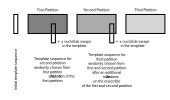
\includegraphics[scale=0.9]{virtual-evolution.pdf}
  \caption{The classic virtual evolution process. The different levels of gray
    show how diffused, (old) the sequences are at the end of the
    process. Please note that $t$ is chosen at random after each
    partition expension.}
  \label{fig-virtual-evolution}
  \end{center}
\end{figure}
\begin{figure}
  \begin{center}
  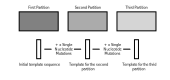
\includegraphics[scale=0.9]{virtual-evolution-controlled.pdf}
  \caption{The more restricted controlled virtual evolution
    process. The different level of gray show how diffused, (old) the
    sequences are at the end of the process. Again note there are
    $M = ptr$ mutations happening across the available sequences after
    each expansion and that $t$ might be variable if chosen so.}
  \label{fig-virtual-evolution-controlled}
  \end{center}
\end{figure}

\subsection{Example}
\lstset{language=bash,
  caption={An example of how to use the \emph{virtual\_evolution} tools.},
  label=lst-virtev-example}
\begin{lstlisting}
virtual_evolution_controlled 42 100 10000 10 -1 1000 4 biosphere.fasta
\end{lstlisting}
In this example the evolutionary process generates 10000 sequences of 100
nucleotides, in 10 partitions of 1000 sequences and a mutation rate
$r=1000$. The time $t=1$, or number of cycles is fixed to one in order
for the diffusion to stay constant during the process. The template
undergoes 4 mutations before creating each new family. The resulting
sequences are stored to \emph{biosphere.fasta}.

\subsection{Implementation}
\emph{virtual\_evolution} and \emph{virtual\_evolution\_controlled}
are implemented in \emph{virtual\_evolution.c} and
\emph{virtual\_evolution\_controlled.c} respectivly. 





\section{simulation\_verification}

\subsection{General}

This is a small tool that tells you how many families created by a virtual
evolution run performed using the tools shown in section
\ref{sec-virtual-ev} can be found by an adaptive clustering run executed using
the tools shown in section \ref{sec-adaptive-clust}. As such this is
an internal quality measurement tool.

\subsection{Usage}

The tool can be run by issuing the following command:

\lstset{language=bash,
  caption={Calling the \emph{simulation\_verification} tool},
  label=lst-simver-call}
\begin{lstlisting}
simulation_verification [fasta] [partitions] [precision] [split-sets]
\end{lstlisting}
with the arguments:
\begin{enumerate}
  \item \emph{fasta} A FASTA file containing a virtual evolution
    dataset as generated with the tools in section
    \ref{sec-virtual-ev}.
  \item \emph{partitions} The number of partitions in the dataset as
    chosen during the virtual evolution run.
  \item \emph{precision} How many sequences have to attributed
    correctly to a family or cluster in order to be proven to be
    correct. If you chose for instance 0.8 here a family of 1000
    sequences can only be found in clusters that have between 800 and
    1200 sequences and hold at least 800 sequences of the of the
    original partition. 
  \item \emph{split-sets} The binary clusters layer files that are the
    result of an adaptive clustering run performed with the tools presented in
    section \ref{sec-adaptive-clust}.
\end{enumerate}

\subsection{Example}
\lstset{language=bash,
  caption={An example of the \emph{simulation\_verification} tool.},
  label=lst-simver-example}
\begin{lstlisting}
simulation_verification sim.fasta 10 0.8 /tmp/s*
\end{lstlisting}
In this example the simulation verification tool uses the simulated dataset
sim.fasta which contains 10 partitions and investigates if clusters found
during an adaptive clustering run yielded at least in one layer the correct
attribution of a family under the precision criteria 0.8.

A possible output might be:
\lstset{language={},
  caption={Example output of the \emph{simulation\_verification}
    tool.},
  label=lst-simver-output-example}
\begin{lstlisting}
Found 8 out of 10 partitions
\end{lstlisting}

\subsection{Implementation}
The tool is implemented in \emph{simulation\_verification.c}.

\section{pca2densitymap} \label{sec-pca2densitymap}

\subsection{General}

The \emph{pca2densiymap} tool allows you to visualize the the sequence density
in a PCA file, as for instance created using the \emph{fasta2kmer} tool
outlined in section \ref{sec-fasta2kmer},
by generating a portable network graphics (PNG) image. This basically 
produces a histogram by laying a rectangular grid across a projection
into two/three dimensional subspace, spun by principal components. The
tool then counts how many sequences are found within a square/cube
and attributes this value to a pixel/voxel in the final
image/images. The 3D version creates a stack of images. To overcome
the limitations of an image based tool such as this one,
one may refer to the \emph{pca2densityfile} tool outlined in section
\ref{sec-pca2densityfile}. 

\subsection{Usage}

The tool can be run using the following commands:
\lstset{language=bash,
  caption={Calling the \emph{pca2densitymap} tool},
  label=lst-pca2densitymap-call}
\begin{lstlisting}
pca2densitymap [fasta] [pca] [dimensions] [2D or 3D] \
  [invertal-length] [png-file-or-files]
\end{lstlisting}
with the arguments:
\begin{enumerate}
  \item \emph{fasta} The original FASTA file that has been transformed
    into a k-mer representation which was projected into a subspace
    spun by principal components. For instance by using the tools
    \emph{fasta2kmer} and \emph{kmer2pca} as described in sections
    \ref{sec-fasta2kmer} and \ref{sec-kmer2pca}.
  \item \emph{pca} A file containing the projections onto the
    principal components.
  \item \emph{dimensions} An integer describing how many dimensions
    the PCA subspace consists of.
  \item \emph{2D or 3D} One may choose 2 for a 2-dimensional output or 3 for a
    3-dimensional output. 3-dimensional outputs are not fully tested
    though.
  \item \emph{interval-length} The grid spacing for our histogram.
  \item \emph{png-file-or-files} A path for the resulting PNG file. In
    case of a 3D output a whole stack of images with individual
    numbers for each slice will be created.  
\end{enumerate}

\subsection{Example}
\lstset{language=bash,
  caption={Example of the \emph{pca2densitymap} tool},
  label=lst-pca2densitymap-example}
\begin{lstlisting}
pca2densitymap test.fasta test.pca 7 2 0.1 /temp/out.png
\end{lstlisting}
In this example an image, \emph{out.png} will be created that contains
pixels ranging from
white, representing the highest number of sequences found in a  grid
tile, to black, with no sequences in the boundaries of a grid
tile. As the image can only encode 8 bits per pixel only 255 different
gray levels are available. This might cause, due to the rescaling,
that only a few white points exist in the image if the dataset
contains very large peaks. \emph{test.fasta} is the sequence
dataset, \emph{test.pca} its projection into a 7 dimensional PCA
subspace. The tool always chooses to only treat either the first two or
three dimensions, for the 2D or 3D case respectively.
Further in this example, we ask for a two dimensional output
with a grid spacing of
0.1 [k-mer frequencies]. The tool yields some information about
the image generated:
\lstset{language={},
  caption={Text output of the \emph{pca2densitymap} tool},
  label=lst-pca2densitymap-txt-out}
\begin{lstlisting}
   shift x:  8.45373440
   shift y:  5.56738997
n points x:    122
n points y:     89
factor 255/maximum(intensity): 0.10814250
\end{lstlisting}
where shift x and y are origin of the image, in general on the upper
left. n Points x and y are the number of pixels according to the
spacing chosen that are calculated and stored in the output PNG
file. The last value is the scalefactor that has been used in order to
scale the densities from 0 to 255. A sample
of an image generated using this tool is highlighted in figure
\ref{fig-pca2densitymap}.
\begin{figure}
  \begin{center}
    \includegraphics{pca-density.png}
    \caption{The sequence density in a two dimensional PCA subspace of
    a k-mer representation. The image was upscaled and color inverted
    for printing using the Gnu Image Manipulation Program (GIMP)
    \cite{gimp}.}
    \label{fig-pca2densitymap}
  \end{center}
\end{figure}

\subsection{Implementation}
The interface to this tool is implemented in \emph{pca2densitymap.c}.
The engine of the tool resides in \emph{density.c}.

\section{pca2densityfile} \label{sec-pca2densityfile}

\subsection{General}

The \emph{pca2densityfile} functions similar to the
\emph{pca2densitymap} tool outlined in section
\ref{sec-pca2densitymap}. It generates a two dimensional histogram
accross a 2 dimensional PCA projection by selection of a grid
spacing. The tool then outputs the densities for each tile to a text
file that can be used for further processing, or external
visualisation tools.

\subsection{Usage}

The \emph{pca2densityfile} tool can be called like:
\lstset{language=bash,
  caption={Calling the \emph{pca2densityfile} tool},
  label=lst-pca2densityfile-call}
\begin{lstlisting}
pca2densityfile [fasta] [pca] [dimensions] [interval-length] > [densityfile]
\end{lstlisting}
with the arguments:
\begin{enumerate}
  \item \emph{fasta} A FASTA file that has been transformed to a k-mer
    representation (i.e. using \emph{fasta2kmer} as shown in section
    \ref{sec-fasta2kmer}) and where such a k-mer representation has been
    projected onto a PCA subspace (i.e. using \emph{kmer2pca} as
    outlined in section \ref{sec-kmer2pca}.
  \item \emph{pca} The projections onto the principal components.
  \item \emph{dimensions} How many principal components have been
    retained, the dimensionaly of the PCA subspace stored in the
    \emph{pca} file.
  \item \emph{interval-length} The grid distance, i.e. the tile size
    of the histogram.
  \item \emph{densityfile} A text file where for each tile a density
    value is stored.
\end{enumerate}

\subsection{Example}
\lstset{language=bash,
  caption={Example of the \emph{pca2densityfile} tool},
  label=lst-pca2densityfile-example}
\begin{lstlisting}
pca2densitymap test.fasta test.pca 7 0.1 > /tmp/out
\end{lstlisting}
In this example a dataset of sequences \emph{test.fasta} and a
representation in a 7 dimensional PCA subspace obtained from a k-mer
representation of the sequences \emph{test.pca} is examined. A
histogram is generated using a grid spacing (tile size) of 0.1
[k-mer frequencies]. How many frequencies are found in each tile is
printed to the output file \emph{/tmp/out}.
\lstset{language={},
  caption={Example output of the \emph{pca2densityfile} tool},
  label=lst-pca2densityfile-output}
\begin{lstlisting}
   shift x:  8.45373440
   shift y:  5.56738997
n points x:    122
n points y:     89
0 0 0
1 0 0
2 0 0
3 0 0
4 0 0
5 0 0
6 0 0
7 0 0
8 0 0
9 0 0
10 0 0
11 0 0
12 0 0
13 0 0
14 0 0
15 0 0
\end{lstlisting}
In the beginning of the output file you can see a shift x and y value
which tells us about the origin of the file, futher it tells you how many
tiles it has generated accroding to the \emph{interval-length}
parameter. This header is followed by the data which is represented as
three values per line. The x and y coordinate ( of the tile ) i.e. the
number of tile that you are in, and the number of sequences in this
square represents the third value. Such a file can then be used with
3rd party visualization software, such as Blender \cite{blender} in
order to inspect the density of sequences in three dimensions. Such an
example image is shown in figure \ref{fig-pca2densityfile}.
\begin{figure}
  \begin{center}
    \includegraphics{pca-density-file.png}
    \caption{The output of \emph{pca2densityfile} visualized with
      Blender \cite{blender}}
    \label{fig-pca2densityfile}
  \end{center}
\end{figure}
We also provide a Blender import script for blender 2.80 and 2.90
in the following:
\lstset{language=python,
  caption={Python script to import the output of the \emph{pca2densityfile} tool into blender},
  label=lst-pca2densityfile-blender}
\begin{lstlisting}
import bpy

def add_map_from_density_file(filename, objname, delta, scalefactor):
    f = open(filename, "r")

    line = f.readline();
    line_array = line.split();
    shift_x = float(line_array[2]);

    line = f.readline();
    line_array = line.split();
    shift_y = float(line_array[2]);

    line = f.readline();
    line_array = line.split();
    n_points_x = int(line_array[3]);

    line = f.readline();
    line_array = line.split();
    n_points_y = int(line_array[3]);

    verticies = [];
    faces = [];

    n_points = n_points_x*n_points_y

    for i in range(n_points):
        line = f.readline()
        line_array = line.split();
        current_point = [(delta*float(line_array[0])-shift_x,
                          delta*float(line_array[1])-shift_y,
                          float(line_array[2])*scalefactor)]
        verticies.extend(current_point)

    for j in range(n_points_y-1):
        for i in range(n_points_x-1):
            current_face = [(j*n_points_x+i,(j+1)*n_points_x+i,
                            (j+1)*n_points_x+i+1,j*n_points_x+i+1)]
            faces.extend(current_face)

    themesh = bpy.data.meshes.new(objname)
    theobject = bpy.data.objects.new(objname, themesh)
    
    bpy.data.objects.new(objname, themesh)
    bpy.context.scene.collection.objects.link(theobject)

    themesh.from_pydata(verticies, [], faces)
    themesh.update(calc_edges=True)

    return theobject

rescale = 5.;

add_map_from_density_file("/tmp/desityfile", "surface-name", 0.1, 0.03/rescale)
\end{lstlisting}
where you have to adapt \emph{/tmp/densityfile} to the location of your
output, \emph{surface-name} to the name that you want to give to your 3D
surface and \emph{0.1} to the grid spacing that you have chosen and
\emph{0.03} to your rescale factor.

\subsection{Implementation}
The interface to this tool is implemented in \emph{pca2denistyfile.c}.
The inner workings are implemented in \emph{density.c}.


\section{reverse\_with\_mask}

\subsection{General}

This tool allows you to reverse selected sequences in a FASTA file. A
mask text file has to be provided to indicate which sequences shall
be reversed. This tool only changes the read direction of the of the
selected sequences. A more elaborate tool is the
\emph{reverse\_complement\_with\_mask} tool found in section \ref{sec-revcomp}.

\subsection{Usage}

The \emph{reverse\_with\_mask} tool can be called like:
\lstset{language=bash,
  caption={Calling the \emph{reverse\_with\_mask\_tool} tool},
  label=lst-revmask-call}
\begin{lstlisting}
reverse_with_mask [fasta] [mask] > [fasta-out]
\end{lstlisting}
with the following arguments:
\begin{enumerate}
  \item \emph{fasta} A FASTA file to reverse sequences in.
  \item \emph{mask} A mask file to indicate the utility which sequences to
    reverse. The file has to contain a line with a number for each
    sequence. If the number matches 1 the sequence corresponding to
    this line in the mask file is reversed in the FASTA output file.
  \item \emph{fasta-out} The FASTA dataset of all sequences
    with those reversed where the mask matches.
\end{enumerate}

\subsection{Example}
Imagine the following FASTA file with three sequences:
\lstset{language={},
  caption={Example of the \emph{reverse\_with\_mask} tool - FASTA file},
  label=lst-revmask-fasta}
\begin{lstlisting}
> sequence_1
ACTG
> sequence_2
ACCT
> sequence_3
GGAT
\end{lstlisting}
As we would like to reverse the second sequence we create the
following mask file:
\lstset{language={},
  caption={Example of the \emph{reverse\_with\_mask} tool - Mask file},
  label=lst-revmask-mask}
\begin{lstlisting}
0
1
0
\end{lstlisting}
Calling the tool as outlined below:
\lstset{language=bash,
  caption={Example of the \emph{reverse\_with\_mask} tool},
  label=lst-revmask-example}
\begin{lstlisting}
reverse_with_mask test.fasta test.mask > out.fasta
\end{lstlisting}
will produce the following FASTA file output:
\lstset{language={},
  caption={Example of the \emph{reverse\_with\_mask} tool - Output FASTA file},
  label=lst-revmask-fastaout}
\begin{lstlisting}
> sequence_1
ACTG
> sequence_2
TCCA
> sequence_3
GGAT
\end{lstlisting}

\subsection{implementation}
The tools interface is implemented in \emph{reverse\_with\_mask.c}.
The code that reverses the sequences resides in \emph{dataset.c}.


\section{reverse\_complement\_with\_mask} \label{sec-revcomp}

\subsection{General}

This tool allows you to reverse complement selected sequences in a FASTA file.
A mask text file has to be provided to indicate which sequences shall
be reversed. This tool not only changes read direction of the
selected sequences but also correctly complements the nucleotides.

\subsection{Usage}

The \emph{reverse\_complement\_with\_mask} tool can be called like:
\lstset{language=bash,
  caption={Calling the \emph{reverse\_complement\_with\_mask\_tool} tool},
  label=lst-revcomp-call}
\begin{lstlisting}
reverse_with_mask [fasta] [mask] > [fasta-out]
\end{lstlisting}
with the following arguments:
\begin{enumerate}
  \item \emph{fasta} A FASTA file to reverse complement sequences in.
  \item \emph{mask} A mask file indicating the utility which sequences to
    reverse complement. The file has to contain a line with a number for each
    sequence. If the number matches 1 on line of the mask file, the
    sequence corresponding to this line is replaced by its reverse
    complement in the resulting FASTA file.
  \item \emph{fasta-out} The FASTA dataset containing all sequences
    together with the reverse complemented at location where the mask matched.
\end{enumerate}

\subsection{Example}
We imagine the following FASTA file with three sequences:
\lstset{language={},
  caption={Example of the \emph{reverse\_complement\_with\_mask} tool -
    FASTA file},
  label=lst-revcomp-fasta}
\begin{lstlisting}
> sequence_1
ACTG
> sequence_2
ACCT
> sequence_3
GGAT
\end{lstlisting}
As we would like to reverse complement the second sequence, we write
a mask file with the following contents:
\lstset{language={},
  caption={Example of the \emph{reverse\_complement\_with\_mask} tool -
    Mask file},
  label=lst-revcomp-mask}
\begin{lstlisting}
0
1
0
\end{lstlisting}
Running the tool by issuing the following command:
\lstset{language=bash,
  caption={Example of the \emph{reverse\_complement\_with\_mask} tool},
  label=lst-revcomp-example}
\begin{lstlisting}
reverse_complement_with_mask test.fasta test.mask > out.fasta
\end{lstlisting}
produces the following \emph{out.fasta} file:
\lstset{language={},
  caption={Example of the \emph{reverse\_complement\_with\_mask} tool -
    Output FASTA file},
  label=lst-revcomp-fastaout}
\begin{lstlisting}
> sequence_1
ACTG
> sequence_2
AGGT
> sequence_3
GGAT
\end{lstlisting}

\subsection{Implementation}
The tools interface is implemented in \emph{reverse\_complement\_with\_mask.c}.
The code that reverses the sequences resides in \emph{dataset.c}.

\section{digest\_X}

The \emph{digest\_X} tools allow you to virtually digest a sequence
using restriction enzymes creating a FASTA file with the sequences
cutted appart. Currently following tools corresponding to the following
restrinction enzymes are implemented: \emph{digest\_XbaI}, \emph{digest\_XmnI}
and \emph{digest\_HindIII}. 

\subsection{Usage}
The tools can be used in the following manner:
\lstset{language=bash,
  caption={Calling the \emph{digest\_X} tools},
  label=lst-digest-call}
\begin{lstlisting}
digest_XbaiI [fasta] [n-threads] > [fasta-out]
digest_XmnI [fasta] [n-threads] > [fasta-out]
digest_HindIII [fasta] [n-threads] > [fasta-out]
\end{lstlisting}
with the arguments:
\begin{enumerate}
\item \emph{fasta} A FASTA file. Only the first sequence of the \emph{fasta}
  file will be digested.
\item \emph{n-threads} How many threads to use for this digestion process.
\item \emph{fasta-out} A fasta file containing the digested sequences.
\end{enumerate}

\subsection{Example}
\lstset{language=bash,
  caption={Example of the \emph{digest\_X} tools},
  label=lst-digest-example}
\begin{lstlisting}
digest_HindIII test.fasta 8 > digested.fasta
\end{lstlisting}
Digests the first sequence stored in \emph{test.fasta} and stores the resulting
sequences in \emph{digested.fasta}. The digestion process can use up to eight
threads on the machine it runs on. The restriction enzyme used for this
virtual digestion is HindIII. 

\subsection{Implementation}
The interface to the \emph{digest\_X} tools is implemented in \emph{digester.c}
The digestion engine is implemented in \emph{restriction\_digest.c}. 

\section{replace\_N\_sequence}


\subsection{General}

\emph{replace\_N\_sequence} Is a tool to replace sequences that are
holding N letters in them with all possible combinations
possible. This tool currently only works with nucleotide sequences.

\subsection{Usage}

The tool can be called like:
\lstset{language=bash,
  caption={Calling the \emph{replace\_N\_sequence} tool},
  label=lst-repnseq-call}
\begin{lstlisting}
replace_N_sequence [fasta] [sequence-index] [fasta-out]
\end{lstlisting}
where the arguments are as follows:
\begin{enumerate}
\item \emph{fasta} A FASTA file holding sequences
\item \emph{sequence-index} An index to select a sequence from the
\item \emph{fasta} file. In this tool the first sequence is selected by
  1.
\item \emph{fasta-out} All possible permutations by replacing the N
  letters in the sequence.
\end{enumerate}

\subsection{Example}
Let us imagine a fasta file like the following:
\lstset{language={},
  caption={Fasta example for the \emph{replace\_N\_sequence} tool},
  label=lst-repnseq-fastaex}
\begin{lstlisting}
>sequence1
ACGT
>sequence2
ANNT
>sequence3
ANTG
\end{lstlisting}
We would like to get all sequences possible by replacing the N letters
in the second sequence, hence we call the utility like:
\lstset{language=bash,
  caption={Fasta example for the \emph{find\_satellite} tool},
  label=lst-repnseq-example}
\begin{lstlisting}
replace_N_sequence test.fasta 2 /tmp/out.fasta
\end{lstlisting}
And get a \emph{/tmp/out.fasta} that looks like:
\lstset{language={},
  caption={Fasta example for the \emph{replace\_N\_sequence} tool},
  label=lst-repnseq-fastaout}
\begin{lstlisting}
>sequence_0
AAAT
>sequence_1
ACAT
>sequence_2
AGAT
>sequence_3
ATAT
>sequence_4
AACT
>sequence_5
ACCT
>sequence_6
AGCT
>sequence_7
ATCT
>sequence_8
AAGT
>sequence_9
ACGT
>sequence_10
AGGT
>sequence_11
ATGT
>sequence_12
AATT
>sequence_13
ACTT
>sequence_14
AGTT
>sequence_15
ATTT
\end{lstlisting}

\subsection{implementation}
The tools interface is implemented in
\emph{replace\_N\_sequence.c}. The mechanism is implemented in
\emph{kmers.c}.



\section{tree\_pureness} \label{sec-pureness}

\subsection{General}

\emph{tree\_pureness} is a tool that can compare a tree and the layer wise
cluster partitions generated by an adaptive clustering run, for
instance, with the tools outlined in section \ref{sec-adaptive-clust}
with a ground trouth set.
Ground trouth sets can for instance be created using the
\newline \emph{split\_set\_from\_annotation} (c.f. section
\ref{sec-ssannotation}) or \newline \emph{split\_set\_from\_swarm}
(c.f. \ref{sec-ssannotation})
tool if a comparison against such tools is the reason for using this
utility. \emph{Tree\_purness} calculates the following tree indices:
\begin{enumerate}
\item Pureness Index,
\item Cluster correspondance,
  and
\item Impure over pure.
\end{enumerate}
This tool is the major tree quality measurement tool in
MNHN-Tree-Tools if the ground truth for a tree is known. 

\subsection{Usage}
The tool can be called like
\lstset{language=bash,
  caption={Calling the \emph{tree\_pureness} tool},
  label=lst-treepureness-call}
\begin{lstlisting}
tree_pureness [fasta] [ground-truth] [split-sets] > [output]
\end{lstlisting}
with the following arguments:
\begin{enumerate}
\item \emph{fasta} A FASTA dataset of sequences that was used to build
  a tree from, and that has a known a ground truth set of partitions.
\item \emph{ground-truth} A binary \emph{split-set} file that contains
  the partitions of the ground truth.
\item \emph{split-sets} The resulting \emph{split-set}s from an adaptive
  clustering run, that represent a full tree. (Such a set can be
  obtained by the tools outlined in section \ref{sec-adaptive-clust}.)
\item \emph{output} The output is a text file containing for each layer in a
  tree all three indices, as outlined above, that enable an efficient
  comparison to a ground truth partition.
\end{enumerate}

\subsection{Algorithm}
The program defines the three indices:
\begin{enumerate}
\item \emph{Pureness:} We define the Pureness Index to be:
  \begin{equation}
    P_{l} =
    \frac{1}{n_{l,\mathrm{inp}}}
    \sum_{i=1}^{n_{l,\mathrm{inp}}}\sum_{k=1}^{n_{\mathrm{target}}}
    \frac{f_{l,i,k}^{<50\%}}{C_{l,i}},
    \label{eqn-pureness}
  \end{equation}
  where $l$ represents the layer of a tree, $n_{l,\mathrm{inp}}$ the
  number of impure clusters and hence, the clusters that are mixture of
  two partitions from the initial truth dataset to compare to.
  $n_{\mathrm{target}}$ is the number of partitions in the original
  truth dataset, $f_{l,i,k}^{<50\%}$ the number of elements
  belonging to partition $k$ of the truth dataset in the impure
  cluster indexed by $i$ in layer $l$ if this number represents less
  then 50\% of the elements in the inpure cluster otherwise
  $f_{l,i,k}^{<50\%}$ represents the total number of elements in the
  impure cluster minus the elements in this cluster that belong to
  the partition of the truth dataset that is indexed by $k$. Finally
  $C_{l,i}$ represents the total number of elements in the impure
  cluster in layer $l$ indexed by $i$.
\item \emph{Cluster correspondance}: It is straight forward to
  reason that pureness as define above is not enough, as a
  partitioning with enough small clusters would yield highly pure
  clusters but not a meaningful partitioning, as such we further
  define:
  \begin{equation}
    S_{l}=\frac{|n_{l}-n_{\mathrm{target}}|}{n_{\mathrm{target}}}, \label{eqn-c-corr}
  \end{equation}
  where $n_{l}$ is the number of clusters in layer $l$ to be the
  measure of correspondance between the number of clusters in the
  truth partioning and the number of clusters obtained in our
  partitioning.
\item \emph{Impureness over pureness}: Finally we argue that we require a
  third value in order to describe the quality of our tree:
  \begin{equation}
    I_{l}=\frac{n_{l,\mathrm{inp}}}{n_{l}}. \label{eqn-impure-pure}
  \end{equation}
  $I_{l}$ represents the number of impure clusters, hence those who
  contain mixtures of partitions from the truth partitioning over
  the number of clusters that are pure.
\end{enumerate}
An example of clustering and the calculation of the three indices is shown
in figure \ref{fig-pureness}.
\begin{figure}
  \begin{center}
  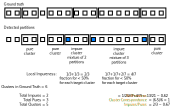
\includegraphics[scale=0.9]{pureness.pdf}
  \caption{A ground truth and a computed clustering. The figure shows how
    the cluster indices: Pureness, Cluster Correspondence and
    Impureness over Pureness are calculated.}
  \label{fig-pureness}
  \end{center}
\end{figure}

\subsection{Example}
We call \emph{tree\_purness} like
\lstset{language=bash,
  caption={Example of the \emph{tree\_pureness} tool},
  label=lst-treepureness-example}
\begin{lstlisting}
tree_purness test.fasta ground-truth /tmp/s* > /tmp/pureness
\end{lstlisting}
where \emph{test.fasta} is a dataset and \emph{ground-truth} is a
binary \emph{split-set} describing the partition we are comparing
all the clusterings in the tree to. \emph{/tmp/s*} is the wildcard to
select all the binary clusterings that have been produced for a
complete tree using an adaptive clustering run (c.f. section
\ref{sec-adaptive-clust}).
A resulting \emph{/tmp/pureness} file might look like the following:
\lstset{language={},
  caption={Example output of the \emph{tree\_pureness} tool},
  label=lst-treepureness-output}
\begin{lstlisting}
0.207187        1.015385        0.259542
0.207658        0.761538        0.288210
0.214303        0.407692        0.267760
0.267122        0.230769        0.281250
0.270319        0.007692        0.297710
0.278394        0.176923        0.280374
0.333774        0.330769        0.264368
0.301733        0.415385        0.315789
0.327885        0.569231        0.267857
\end{lstlisting}
The output presents three tabulator separated values per line, where
the first value
is the Pureness, the second the Cluster Correspondence and the third
the Impureness over Pureness value. Using a tool like
\emph{gnuplot} for instance one can create a three value diagram in
order to judge if a level of
the tree yields the accuracy requested to the ground truth. Such an
example is shown in figure \ref{fig-pureness-example}.
\begin{figure}
  \begin{center}
    \includegraphics[scale=1.4]{pureness-example.pdf}
    \caption{An example of a visual representation of the data
      obtained from the \emph{tree\_pureness} tool. On the abscissa
      the $\epsilon$ values shown reside in the output of
      the adaptive clustering run (c.f. section \ref{sec-adaptive-clust}).}
    \label{fig-pureness-example}
  \end{center}
\end{figure}

\subsection{Implementation}
The interface is implemented in \emph{tree\_purness.c}. The
functionality is to be found in \emph{cluster\_io.c}. 






\appendix
%\input{appendix}

\bibliography{bib}{}
\bibliographystyle{vancouver}

\end{document}
